%\documentclass[a4paper,12pt,ngerman,fleqn,bibtotoc]{article}
\documentclass[liststotoc,bibtotoc,fontsize=12pt,paper=a4,titlepage,twoside,DIV=10,notitlepage]{scrartcl} %scrartcl scrreprt article  scrbook

% redefine reprt to article (see: http://www.golatex.de/scrreprt-chapter-immer-auf-einer-neuen-seite-t2420.html#9047)
\let\chapter\section
\let\section\subsection
\let\subsection\subsubsection
\let\subsubsection\paragraph
\let\paragraph\subparagraph
\let\subparagraph\undefined 
% end

\usepackage[english,ngerman]{babel}
\usepackage[utf8]{inputenc}

% Farbumgebung fuer Latex und Textboxen
\usepackage[usenames]{color}

\usepackage{typearea}

\usepackage{texdraw}
\usepackage{graphicx}
\usepackage{fancyhdr} % Seitengestaltung - Header / Body mit Überschriften
\usepackage{fancyvrb} % Nummerierung von verbatim

\usepackage{supertabular}
\usepackage{longtable}
\usepackage[right]{eurosym}
\usepackage{a4wide}
\usepackage{graphicx}
%\usepackage{picins}
\usepackage{array}
\usepackage{ae} % Schöne Schriften für PDF-Dateien
\usepackage{lmodern} % Latin Modern


\usepackage{listings}
  %\lstset{numbers=left, numberstyle=\tiny, numbersep=5pt}
  %\lstset{language=bash}
  \lstset{
	basicstyle=\ttfamily\fontsize{9pt}{10pt}\selectfont,
	language=bash,			% choose the language of the code
	numbers=left,			% where to put the line-numbers
	%numberstyle=\tiny,		% the size of the fonts that are used for the line-numbers
	stepnumber=2,			% the step between two line-numbers. If it's 1 each line will be numbered
	emptylines=*1,			% If there is a block of more than number (*) empty lines, only number (1) ones are printed.
	breaklines=true,                % sets automatic line breaking
	breakatwhitespace=false,        % sets if automatic breaks should only happen at whitespace
	showspaces=false,               % show spaces adding particular underscores
	showstringspaces=false,         % underline spaces within strings
	showtabs=false,                 % show tabs within strings adding particular underscores
	frame=none,			% adds a frame around the code
	columns=fixed,			% The (alignment) can be fixed, flexible, spaceflexible or fullflexible
	escapechar={§},			% If not empty the character escapes to LATEX
	extendedchars=true,		% allows or prohibits extended characters in listings, that means (national) characters of codes 128–255.
	commentstyle=\color{red},
	%directivestyle=\color{green},
	stringstyle=\color{gray},
	%backgroundcolor=\color{lightgray},
	keywordstyle=\bf\color{blue},
	captionpos=b,                   % sets the caption-position to bottom
%	aboveskip=10pt			define the space above the listing
%	belowskip=10pt			define the space below the listing
	lineskip=3pt			% additional space between lines in listing
  }

\lstdefinelanguage{conf} {
   basicstyle=\ttfamily\fontsize{9pt}{10pt}\selectfont\color{black},
   sensitive=true,
   escapechar={§},
%    escapeinside={(*@}{@*)},
%    morecomment=[s][\color{red}\ttfamily]{<--}{-->}, commentstyle=\color{red},
%    showstringspaces=false,
%    numberstyle=\scriptsize,
%    numberblanklines=true,
%    showspaces=false,
   breaklines=true,
   stepnumber=2,			% the step between two line-numbers. If it's 1 each line will be numbered
%    showtabs=false,
  backgroundcolor=\color{lightgray}
}

\lstdefinelanguage{data} {
   basicstyle=\ttfamily\fontsize{9pt}{10pt}\selectfont\color{black},
   sensitive=true,
   escapechar={§},
numbers=none,
%    escapeinside={(*@}{@*)},
%    morecomment=[s][\color{red}\ttfamily]{<--}{-->}, commentstyle=\color{red},
%    showstringspaces=false,
%    numberstyle=\scriptsize,
%    numberblanklines=true,
%    showspaces=false,
   breaklines=true,
   stepnumber=2,			% the step between two line-numbers. If it's 1 each line will be numbered
%    showtabs=false,
  backgroundcolor=,
%  belowskip=0pt
}

\usepackage[font=small,format=plain,labelfont=bf,up,textfont=it,up]{caption} % Bildunterschriften formatieren

\usepackage{empheq}

%Fixme Notizen anbringen
\usepackage[
inline, %Setzt Notiz direkt in den Text
%margin, %Setzt Notiz an den Rand (default)
%marginclue %Setzt nur einen Hinweis an den Rand
]{fixme} 

% ToDo Notes
\usepackage[]{todonotes}
% examples:
% \missingfigure{hier fehlt n Bild}
% \todo[inline]{blah}

\usepackage{paralist} % itemize Listing erweitern sodass Aufzaehlungszeichen geaendert werden koennen
% Beispiel:
%\begin{itemize}
%\item[$\filledtriangleright$] blah
%\item[$\filleddiamond$] blubb
%\item[$\smalltriangleright$] fasel
%\end{itemize}

\usepackage{MnSymbol} % Mathematische Symbole includen

\usepackage{colortbl}	% Farben fuer Tabellen

%\parindent0mm % Legt die EinrückTiefe der ersten Zeile für alle folgenden Absätze fest



% Glossar Package einbinden
%\usepackage{glossaries}
%\usepackage{makeglos}
%\usepackage{glossary}

\usepackage[
nonumberlist, %keine Seitenzahlen anzeigen
acronym=false,      %ein Abkürzungsverzeichnis erstellen
toc,          %Einträge im Inhaltsverzeichnis
section]      %im Inhaltsverzeichnis auf section-Ebene erscheinen
{glossaries}


%\usepackage{breakurl}
\usepackage[      % Links in PDF Dokumenten - MUSS immer als letztes eingebunden werden !!!
colorlinks=true,
linkcolor=blue,
bookmarks=true,
pdffitwindow=true,
plainpages=false,
%linktocpage=true,	%Links im Inhaltsverzeichnis Table of Contents
%frenchlinks=false,
breaklinks=true]
{hyperref}

% Farbumgebung fuer Latex und Textboxen
\definecolor{green}{rgb}{0.0,0.7,0.0}
\definecolor{black}{rgb}{0.0,0.0,0.0}
\definecolor{blue}{rgb}{0.0,0.0,0.75}
\definecolor{gray}{rgb}{0.30,0.30,0.30}
%\definecolor{lightgray}{rgb}{0.91,0.91,0.91}
\definecolor{ulgray}{rgb}{0.95,0.95,0.95}
\definecolor{red}{rgb}{1.0,0.0,0.0}
\definecolor{brown}{rgb}{0.5,0.0,0.0}
\definecolor{lightblue}{rgb}{0.6,0.75,0.95}
\definecolor{lightgreen}{rgb}{0.6,0.95,0.65}
\definecolor{lightred}{rgb}{0.95,0.75,0.6}
\definecolor{cstred}{rgb}{0.94,0.5,0.5}
\definecolor{lightyellow}{rgb}{0.95,0.95,0.6}
\definecolor{lightmagenta}{rgb}{0.95,0.6,0.95}
\definecolor{purple}{rgb}{0.65, 0.12, 0.82}



% JavaScript highlighting 
% http://lenaherrmann.net/2010/05/20/javascript-syntax-highlighting-in-the-latex-listings-package
\lstdefinelanguage{JavaScript}{
  keywords={typeof, new, true, false, catch, function, return, null, catch, switch, var, if, in, while, do, else, case, break}
  keywordstyle=\color{blue}\bfseries,
  ndkeywords={class, export, boolean, throw, implements, import, this},
  ndkeywordstyle=\color{darkgray}\bfseries,
  identifierstyle=\color{black},
  sensitive=false,
  comment=[l]{//},
  morecomment=[s]{/*}{*/},
  commentstyle=\color{purple}\ttfamily,
  stringstyle=\color{red}\ttfamily,
  morestring=[b]',
  morestring=[b]"
}


\lstset{
   language=JavaScript,
   %backgroundcolor=\color{lightgray},
   extendedchars=true,
   basicstyle=\footnotesize\ttfamily,
   showstringspaces=false,
   showspaces=false,
   numbers=left,
   numberstyle=\footnotesize,
   numbersep=9pt,
   tabsize=2,
   breaklines=true,
   showtabs=false,
   captionpos=b
}


\makeatletter
\def\url@leostyle{%
  \@ifundefined{selectfont}{\def\UrlFont{\sf}}{\def\UrlFont{\footnotesize\ttfamily}}}
\makeatother
\urlstyle{leo}

\makeatletter
\lst@AddToHook{TextStyle}{\let\lst@basicstyle\ttfamily\small}
\makeatother

\pdfadjustspacing=1


% Kopfzeile erstellen, Seitennummerierung
%\pagestyle{headings}
%\pagestyle{fancy}
%\lhead[\fancyplain{}{\sffamily{}}]%
%      {\fancyplain{}{\sffamily \small{\leftmark}}}
%\rhead[\fancyplain{}{\sffamily \small{\rightmark}}]%
%      {\fancyplain{}{\sffamily{}}}
%\lfoot[\fancyplain{}{\thepage}]%
%      {\fancyplain{}{}}
%\rfoot[\fancyplain{}{}]%
%      {\fancyplain{}{\thepage}}
%\cfoot{}

%Glossar - Den Punkt am Ende jeder Beschreibung deaktivieren
\renewcommand*{\glspostdescription}{}
%Glossar-Befehle anschalten
\makeglossaries

% Glossar File einbinden
%
%
% Glossar
%
\newglossaryentry{AIISO}{
name={Academic Institution Internal Structure Ontology (AIISO)},
description={Ontologie für die Beschreibung der Struktur akademischer Einrichtungen}
}

\newglossaryentry{CSV}{
name={Character Separated Values (CSV)},
description={Format bei dem die einzelnen Elemente durch spezielle Zeichen, z.B. Strichpunkte, getrennt werden}
}

\newglossaryentry{DC}{
name={Dublin Core (DC)},
description={Sammlung von Metadatenelementen zu Beschreibung von Dokumenten/Ressourcen}
}

\newglossaryentry{DAML}{
name={DARPA Agent Markup Language (DAML)},
description={Auszeichnungssprache für das Semantic Web}
}
%\newacronym{EBNF}{EBNF}{Erweiterte Backus-Naur-Form\protect\glsadd{glos:EBNF}}
\newglossaryentry{EBNF}{
name={Erweiterte Backus-Naur-Form (EBNF)},
description={Formale Metasyntax zur Darstellung kontextfreier Grammatiken}
}

\newglossaryentry{F-Logic}{
name={Frame Logic (F-Logic)},
description={Formale Sprache zur Formulierung von Ontologien}
}

\newglossaryentry{FOAF}{
name={Friend of a Friend (FOAF)},
description={Ontologie formalisiert in RDF-Schema für maschinenlesbare Modellierung sozialer Netzwerke}
}

\newglossaryentry{INKIDU}{
name={INKIDU},
description={Inkidu ist ein an der HS Ravensburg-Weingarten entwickeltes Internet Umfragesystem},
first={INKIDU},
text={}
}

\newglossaryentry{HIS}{
name={Hochschul-Informations-System (HIS)},
description={Softwarehaus mit Sitz in Hannover, Entwickler des LSF}
}

\newglossaryentry{KOS}{
name={Knowledge Organization Systems (KOS)},
description={Ein KOS oder Begriffssystem fasst Begriffe oder Klassen aus abgetrennten System zusammen.}
}

\newglossaryentry{LSF}{
name={Lehre, Studium, Forschung (LSF)},
description={Verwaltungsportal für Hochschulen mit Stundenplänen, Prüfungsplänen uvm.}
}
 
\newglossaryentry{Metadaten}{
name={Metadaten},
description={Daten über Daten, Daten welche den Inhalt näher beschreiben},
first={Metadaten},
text={}
}

\newglossaryentry{Microformats}{
name={Microformats},
description={Microformats ist ein Markup-Format für die semantische Beschreibung von (X)HTML Webseiten},
first={Microformats},
text={}
}

\newglossaryentry{OIL}{
name={Ontology Inference Layer (OIL)},
description={Webbasierte Auszeichnungssprache für das Semantic Web}
}

\newglossaryentry{Ontologie}{
name={Ontologie},
description={Menge von Begrifflichkeiten und deren Beziehungen für eine bestimmte Domäne},
first={Ontologie},
text={}
}

\newglossaryentry{OWL}{
name={Web Ontology Language (OWL)},
description={Beschreibt Zusammenhänge zwischen Termen in RDF}
}

\newglossaryentry{Pattern-Matching}{
name={Pattern-Matching},
description={Sucht nach einem bestimmten vorgegebenen Muster in einer diskreten Struktur},
first={Pattern-Matching},
text={}
}

\newglossaryentry{RDF}{
name={Resource Description Framework (RDF)},
description={Framework für die Beschreibung von Objekten (Ressourcen) und deren Eigenschaften in Triples}
}

\newglossaryentry{RDFS}{
name={RDF-Schema (RDFS)}, description={Erweitert RDF und formalisiert einfache Ontologien für eine Domäne}
}

\newglossaryentry{REST}{
name={Representational State Transfer (REST)}, description={Architektur für verteilte Anwendungen, beispielhaft dafür ist das World Wide Web}
}

\newglossaryentry{RESTful}{
name={RESTful}, description={Erfüllt die Anforderungen an einen REST Webservice}
first={RESTful},
text={}
}

\newglossaryentry{SKOS}{
name={Simple Knowledge Organization System (SKOS)},
description={Auf RDF basierende Sprache zur Formalisierung von Klassifikationen und Thesauri}
}

\newglossaryentry{SPARQL}{
name={SPARQL Protocol and RDF Query Language (SPARQL)},
description={Graph-basierte Abfragesprache für RDF}
}

\newglossaryentry{triple store}{
name={triple store},
description={Speichert RDF Metadaten in einer Art Relationalen Datenbank}
first={triple store},
text={}
}

\newglossaryentry{URI}{
name={Uniform Resource Identifier (URI)},
description={Identifikator um jegliche Ressource im WWW eindeutig zu identifizieren}
}

\newglossaryentry{W3C}{
name={World Wide Web Consortium (W3C)},
description={Standardisierungsgremium für das World Wide Web}
}

\newglossaryentry{WOT}{
name={Web of Trust (WOT)},
description={Mit Hilfe einer Community wird ein Vertrauensnetzwerk aufgebaut, um Webseiten und Inhalte als nicht gefährlich einzustufen und um Personen zu authentifizieren.}
}

\newglossaryentry{XML}{
name={XML},
description={eXtensible Markup Language, Auszeichnungssprache für hierarchische Daten}
}




\begin{document}
%\frontmatter
\pagestyle{plain}
%\frontmatter
  % %\lhead{\sc{Dokublah}}
% \title{foo bar}
% %\project{123}
% %\version{200807}
% %\prerequisite{Lastenheft}
% %\prerequisiteref{http://foo.bar/blah.pdf}
% %\author{Andreas Kimpfler}
% %\home{Kisslegg}
% %\homeref{http://foo.bar} 
% 
% 
% 
% % Title Page
% \title{Diplomarbeit \\
% Erstellen eines Migrationsleitfadens auf OpenLDAP Version 2.4 unter Berücksichtigung von Overlay Techniken einschließlich Roll-Out im Produktivsystem der HRW }
% \author{Andreas Kimpfler}
% \date{03.08.2009}
% 
% % Titel erstellen
% \maketitle

\begin{titlepage}
	\areaset[0cm]{21cm}{29cm}
	\vspace*{2cm}
	\begin{center}
		%\vspace{1cm}
		%\\
		
\includegraphics[width=8.0cm]{images/HS-Logo} \\
		 \vspace{2cm}

		\Huge
		\textbf{Informationsmanagement mit XML} \\

		\vspace{1.5cm}

		\huge
		Praktischer Ansatz zur Entwicklung einer \\ Anwendung mit Semantik Web Techniken\\
		%\vspace{2cm} \\
		
		\large
		\vspace{1cm}
		
		\small
		02. Juli 2010 \\		

		

		\vspace{6.5cm}
		Erstellt von: \\ \vspace{0.5cm}
		\textbf{Karl Glatz, 20570} \\ {\small Hochschule Ravensburg-Weingarten} \\
		\vspace{0.3cm}
		\textbf{Sebastian Wiedenroth, 20006} \\ {\small Hochschule Ravensburg-Weingarten} \\
		\vspace{0.3cm}
		\textbf{Benjamin Merkle, 20569} \\ {\small Hochschule Ravensburg-Weingarten}\\
		\vspace{0.3cm}
		\textbf{Andreas Kimpfler, 21027} \\ {\small Hochschule Ravensburg-Weingarten}
	\end{center}
% 	\vfill
\end{titlepage} \newpage
\cleardoublepage
  \chapter*{Erklärung}
Diese Arbeit wurde an der Hochschule Ravensburg-Weingarten als Hausarbeit im Rahmen der Vorlesung ``\textsf{Informationsmanagement mit XML}'' angefertigt.
\\ \\
Hiermit versichern wir, die vorliegende Ausarbeitung und Implementierung selbständig angefertigt und dabei nur die angegebenen Quellen und Hilfsmittel verwendet zu haben.
\\ \\
Die Arbeit wurde bisher in gleicher oder ähnlicher Form keiner anderen Prüfungsbehörde vorgelegt und auch nicht veröffentlicht.
\\ \\ \\ \\ \\
Weingarten, 02. Juli 2010 \hspace{0.5cm}
\begin{tabular}[t]{p{4.5cm}}
 \\
 \hline
 Karl Glatz
 \\ \\
 \hline
 Sebastian Wiedenroth
 \\ \\
 \hline
 Benjamin Merkle
 \\ \\
 \hline
 Andreas Kimpfler
\end{tabular} \newpage
\cleardoublepage 

%\pagestyle{fancy}

% Inhaltsverzeichnis
\tableofcontents

% Fügt manuell einen Verzeichniseintrag in das Inhaltsverzeichnis das Verzeichnis der Abbildungen oder das Verzeichnis der Tabellen ein;  der Eintrag wird automatisch mit der zugehörigen Seitennummer versehen. Solche manuellen Einträge sind besonders dann erforderlich,  wenn man einen Gliederungsbefehl verwendet, der einen solchen Eintrag nicht automatisch erzeugt
\addcontentsline{toc}{section}{Inhaltsverzeichnis} %chapter

  \chapter*{Abstract}

\begin{abstract}
\textsl{Es gibt viele Ansätze und Forschungsprojekte, die das Semantic Web voran\-treiben wollen. Dennoch gehören Technologien des Semantic Web längst nicht zum Alltagswerkzeug eines Webentwicklers. Diese Arbeit gibt einen Überblick über einige Techniken und verwendet diese im Rahmen einer Beispiel-Anwendung zur Evaluierung von Praktikumsstellen für Studenten des Studiengangs Angewandte Informatik. In der Anwendung kommen verschiedene Techniken aus dem Semantic Web Umfeld zum Einsatz. Die für die Anwendung benötigten Daten werden dabei aus internen Datenbanken, dem Umfragesystem, sowie dem Verwaltungsportal für die Vorlesungen der Hochschule entnommen und aufbereitet. Die gesammelten Daten werden semantisch Aufbereitet im Web zur (freien) Verfügung gestellt. Die von uns entwickelte Ontologie versucht möglichst große Teile standardisierter Ontologien zu verwenden. Die Beispiel-Anwendung verwendet Methoden aus der künstlichen Intelligenz um die Daten zu Klassifizieren.}
\end{abstract}

\selectlanguage{english}
\begin{abstract}

\textsl{There are many approaches and research projects that intend to push the Semantic Web. However semantic web technologies are not yet part of the average web developers toolset. This paper gives an overview of some techniques and uses them as a part of an example application for the evaluation of internships for students studying applied computer science. Different semantic web techniques are used in the application. The data needed for the application comes from internal databases, the survey system, and in addition from the management portal for the lectures of the university and get prepared for further use. We publish the resulting semantic data to the world wide web for free use. The developed ontology uses well known ontology standards where possible. The application uses methods from artificial intelligence to classify the data.}
\end{abstract}

\selectlanguage{ngerman}


 \newpage
\cleardoublepage
%\mainmatter
\pagestyle{fancy}
%\part{Einführung}


\chapter{Einleitung}
\label{cap-einleitung}
\section{Motivation und Zielsetzung} % karl
%Die Aufgabenstellung im Fach \textit{Informationsmanagement mit XML} war es, eine Beispielanwendung mit Hilfe von semantischen Web Hochschulwebseiten (klingt kacke, weglassen??)

Über das Semantic Web gibt es bereits zahllose theoretische Arbeiten und Bücher. Auch an der Hochschule Ravensburg-Weingarten wurde in den letzten Jahren mehr über das Semantic Web geschrieben, als dass eine Projektgruppe versucht hat diese Technologien in einem Projekt praktisch umzusetzen. Daher ist die praktische Betrachtung der Technologien für uns besonders von Bedeutung. Dies manifestiert sich neben dem Titel dieser Ausarbeitung auch in der Aufteilung des Dokuments.

Neben dem kurzen Kapitel Grundlagen (\ref{cap-grundlagen}) stellen wir direkt die Projektidee vor (\ref{cap-projektidee}). Im Verlauf dieses Kapitels folgt eine Analyse der Idee im Bezug auf benötigte und verfügbare Daten sowie deren Formate (\ref{sec-analyse-daten}). Im Abschnitt \ref{sec-open-linked-data-hs} wird erläutert wie es um die Verfügbarkeit von semantischen Daten an der Hochschule bestellt ist. Dies ist deswegen so wichtig, weil es sich direkt auf das Ziel unseres Projektes auswirkt. Der Abschnitt Analyse skizziert die \gls{Ontologie} (\ref{sec-idee-datenmodel}) für die Hochschuldaten und anschließend rückt der Fokus auf die Umsetzung dieser Idee. In der Umsetzung (\ref{cap-umsetzung}) werden Toolkits und Frameworks zum einfachen Arbeiten mit Sematic Web Technologien im Einsatz beschrieben (\ref{sec-daten-python} und \ref{sec-daten-joseki}). Abschließend fassen wir unsere Ergebnisse zusammen (\ref{sec-fazit}) und geben einen kurzen Ausblick (\ref{sec-ausblick}).

%, der versucht vom konkreten Projekt den Bogen auf die allgemeine Entwicklung des Semantic Web zu spannen.
%Beleuchtet wird neben den Programmen und Sprachen () auch die Hürden im Projekt (TODO), vor allem im Bezug auf die Verfügbarkeit von Daten.

\section{Arbeitsverteilung}

\begin{table}[h!]
\centering
\begin{tabular}{|l|l|l|}
\hline \textbf{Name} & \textbf{Kapitel/Abschnitt} & \textbf{Weitere Aufgaben} \\ 
\hline Benjamin Merkle & \ref{cap-grundlagen}; \ref{klassifizierung}; Glossar & Diagramme  \\ 
\hline Karl Glatz & \ref{cap-einleitung}; \ref{sec-grundlagen-einf-semweb}; \ref{cap-projektidee} & Konzeption, Konfiguration, JavaScript \\  %Koordination %(\ref{sec-idee-datenquellen} \ref{sec-idee-hintergrund})
\hline Sebastian Wiedenroth & \ref{sec-sparql}; \ref{sec-idee-datenmodel}; \ref{cap-umsetzung} & Konzeption, Python Code, JavaScript \\ 
\hline Andreas Kimpfler & Abstract; \ref{sec-algo}; \ref{cap-zusafa} & Dokument-Style, Server, Dummy Daten \\  %\ref{cap-zusafa}
\hline 
\end{tabular}

\caption{Arbeitsverteilung der Projektteilnehmer}
\end{table}



% % Beispiele für Glossar
%dududu \gls{glos:AntwD} dadada \gls{citrusfruit} und \gls{AD} dudu \gls{EBNF}
%lalala sdfsdf \gls{Metadaten}
%\glsdisp{CATIA}{CATIA} V5

%
% Grundlagen Kaptiel
% Zielsetzung: Techniken erklären und zum Projekt hinführen!
%
\chapter{Semantik Web Grundlagen}
\label{cap-grundlagen}
\section{Einführung: Semantic Web und Linked Data} % karl
\label{sec-grundlagen-einf-semweb}
Oft gelesen, selten verstanden. Das \textbf{Semantic Web} ist kein neues Web, es kann wie das Web 2.0 nur als eine Erweiterung aufgefasst werden. Dabei ist diese nur zu einem geringen Teil technischer Natur. Die grundlegenden, technischen Konzepte und Ideen bestehen inzwischen einige Zeit. Auch deren Umsetzung ist in der Informatik-Zeitrechnung fast schon Geschichte. Trotzdem gibt es kaum Anwendungen, die wirklich Gebrauch vom Semantic Web machen. Dies begründet sich vor allem darin, dass es bisher wenige Informationen als so genannte \textbf{Linked Data} (verknüpfte Daten) gibt, was sich jedoch von Tag zu Tag ändert. Weitere Gründe für die verhaltene Entwicklung in der sonst so von Trend und Boom bestimmten IT-Branche ist auch die technische Akzeptanz, z.B. ist RDF nicht direkt intuitiv zu begreifen.


Im Folgenden werden wir von simplen Begriffserklärungen bis hin zu Projekten, die sich den unterschiedlichsten Aufgabenstellungen des Semantic Web widmen, beleuchten.

% Denn hier handelt es sich - wie so oft - um ein klassisches Henne-Ei-Problem\footnote{\url{http://de.wikipedia.org/wiki/Henne-Ei-Problem}}.


\paragraph*{Semantic Web} 
Erweiterung des World Wide Webs. Im Web veröffentlichte Daten sollen durch Standardformate für Maschinen les- und verarbeitbar werden. Ursprung dafür ist der Artikel \cite{Bern01} des Web-Begründers Tim Berners-Lee.
Wikipedia schreibt (\cite{WPSEMWEB}):
\begin{quote}
``Die Informationen im Web sollen von Maschinen interpretiert und automatisch maschinell weiterverarbeitet werden können. Informationen über Orte, Personen und Dinge sollen mit Hilfe des Semantischen Webs von Computern miteinander in Beziehung gesetzt werden können. [...] Bei der Verknüpfung der Informationen in einem Semantischen Web können neue Zusammenhänge entdeckt werden, die zuvor nicht erkennbar waren.''
\end{quote}


\paragraph*{Linked Data} % andreas
\label{linked-data}
Fachbegriff eines bewährten Verfahrens (best practice) zur Beschreibung von Quellen. Das Verfahren definiert die Darstellung, den Zugriff und die Verbindungen der einzelnen Teilstücke von Daten, Informationen und Wissen zu einem großen Ganzen, dem Semantic Web. Das Zusammenfügen erfolgt dabei mittels \gls{URI} und dem \gls{RDF}.

% a term used to describe a recommended best practice for exposing, sharing, and connecting pieces of data, information, and knowledge on the Semantic Web using URIs and RDF." \todo[inline]{Auf deutsch und überarbeiten; Quelle en.wp} 

Die folgende Abbildung \ref{graphic-lod-datasets} zeigt an einem Beispiel, anhand verschiedenster Datenquellen, wie der Zugriff und die Verbindungen erfolgen und wie man dies in einem Graphen darstellen kann.

\newpage
\begin{figure}[htbp]
	\centering
	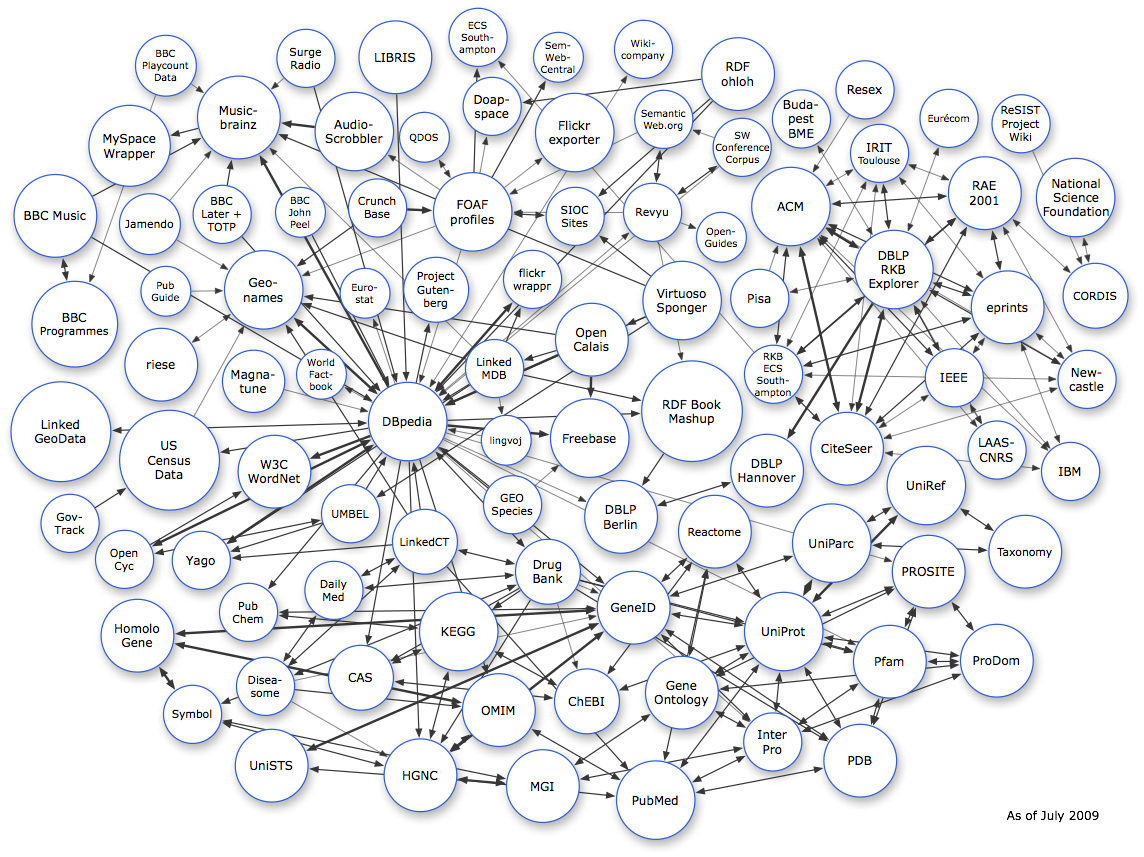
\includegraphics[scale=0.3]{images/lod-datasets_2009-07-14}
	\caption{Linking Open Data: Offene Datenquellen und deren Verbindungen; Quelle: \cite{LINKEDATA}}
	\label{graphic-lod-datasets}
\end{figure}

\section{Triples} % benny 
\label{sec-triples}
Ein Triple besteht im Bezug auf Semantic Web und insbesondere im Bezug auf RDF und OWL aus den drei Elementen Subjekt, Prädikat und Objekt. Die Idee dahinter ist, dass eine Ressource über Subjekte oder Klassen verfügen kann, die bestimmte Eigenschaften haben.
Das Subjekt wird mittels einer \gls{URI} identifiziert. Es kann sich dabei um ein Dokument, einen Gegenstand oder eine Information handeln. Die Eigenschaft, welche eine Ressource hat ist das Prädikat und der Wert dieser Eigenschaft ist das Objekt. Prädikate und Objekte können Zeichenketten sein, aber auch andere Ressourcen. So kann eine rekursive Struktur aufgebaut werden. Ein Triple wird öfters auch Statement genannt.
Eine Möglichkeit Triples darzustellen, zu übertragen oder zu speichern, bietet das N-Triples Format. Dieses zeilenbasierte Format serialisiert das RDF-Format als Klartext. Dieses Format wurde 2004 als offizielle Recommendation vom \gls{W3C} verabschiedet. Turtle ist noch eine Erweiterung von N-Triples, da diese zu wenig Funktionalität bieten. Beispielsweise wurde eine Kurzschreibweise hinzugefügt. Beide Formate sind im wesentlichen Teil des von Tim Berners-Lee vorgeschlagenen Formats N3 (Notation 3), aber beide beschränken sich darauf nur zulässige RDF-Graphen darzustellen. 

\section{RDF}
\gls{RDF} ist ein Framework um Informationen/Metadaten über bestimmte Informationen zu speichern. RDF speichert also sozusagen „Daten über Daten“ (über Daten). Die beschriebenen Informationen sind meist Webressourcen. Dabei spielt es keine Rolle ob die Daten nur einfache Informationen sind oder ein komplexes Objekt. Zum Beispiel können Informationen über den Autor oder das Erstellungsdatum eines Dokuments dargestellt und Informationen über den Inhalt des Dokumentes selber beschrieben werden. Das Hauptziel ist mittels RDF Metadaten automatisch auszuwerten und zu bearbeiten. Weitere Ziele sind das Auffinden von Informationen im Web (Katalogisierung) und Bewertungen von Inhalten (Rating). Außerdem ist RDF ein Baustein des \gls{WOT}, dabei werden über eine Community Webseiten als sicher vermerkt. RDF bietet zusätzlich eine gute Interoperabilität zwischen verschiedenen Metadaten-Systemen.
RDF wird vom W3C bereits seit 1999 entwickelt und ist offen für weitere Erweiterungen.
Das RDF-Framework verwendet die in \ref{sec-triples} Triples um die Informationen zu beschreiben.

\begin{lstlisting}[language=xml,numbers=none,caption=Beispiel für ein einfaches RDF-Dokument,label=code-rdf-grundlage-1]

<?xml version="1.0"?>
<rdf:RDF xmlns:rdf="http://www.w3.org/1999/02/22-rdf-syntax-ns#"
             xmlns:contact="http://www.w3.org/2000/10/swap/pim/contact#">

  <contact:Person rdf:about="http://www.w3.org/People/EM/contact#me">
    <contact:fullName>Eric Miller</contact:fullName>
    <contact:mailbox rdf:resource="mailto:em@w3.org"/>
    <contact:personalTitle>Dr.</contact:personalTitle> 
  </contact:Person>

</rdf:RDF>
\end{lstlisting}
Im Codelisting \ref{code-rdf-grundlage-1} (entnommen aus \cite{RDF-Prim}) findet sich ein kurzes Beispiel für die Beschreibung der Person \flqq Eric Miller\flqq\ in RDF-XML. Darin enthalten sind URIs, welche Ressourcen im Web identifizieren können, Eigenschaften (properties) wie z.B. ``mailbox'' oder ``fullname'' und die Werte der Eigenschaften (values) z.B. ``Eric Miller''. Die XML Elemente werden auch Terms genannt.
Der zugehörige Graph ist in \ref{graphic-rdf-bsp-graph} abgebildet. 
\begin{figure}
	\centering
		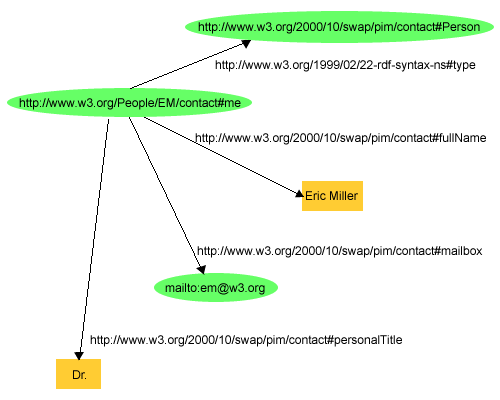
\includegraphics[keepaspectratio,scale=0.6]{images/RDF-bsp}
	\caption{Darstellung des Beispielgraphen}
	\label{graphic-rdf-bsp-graph}
\end{figure}

Durch die Verknüpfung von Daten in Anwendungen werden die Zusammenhänge maschinenlesbar dargestellt. Diese Zusammenhänge können dazu verwendet werden, um dem User weitere Hilfen oder Informationen zu bieten.
\\
Die wichtigsten Eigenschaften von RDF sind:
\begin{itemize}
\item Unabhängigkeit
Jede Domäne kann eigene Prädikate für ihre Subjekte definieren.
\item Austauschbarkeit
Durch die Verwendung von \gls{XML} wird der Austausch und die Kommunikation, zwischen Anwendungen oder Domänen, erheblich vereinfacht.
\item Skalierbarkeit 
Große Mengen von Daten können durch die Einteilung in Triples schnell und effizient verarbeitet werden.
\item Prädikate sind Ressourcen
Durch den rekursiven Aufbau können Prädikate eigene Prädikate haben, welche automatisch weiterverarbeitet werden.
\item Objekte können Ressourcen sein
Wie bei den Prädikaten gilt hier auch der rekursive Aufbau, damit auch diese wieder eigene Ressourcen sein und weiterverarbeitet werden können.
\end{itemize}
Das Ganze hat den Vorteil, dass sich die Daten aus verschieden Anwendungen exportieren lassen, ohne das die Daten der Daten ihre Bedeutungen verlieren.
RDF selbst definiert kein Vokabular für die Beschreibung der Meta Daten, dafür eignet sich beispielsweise \gls{DC}.
Noch zu erwähnen ist, dass RDF nicht durch eine XML DTD definiert ist sondern durch die \gls{EBNF}. Dadurch ist RDF unabhängig von XML.

\paragraph{RDF Syntax}
RDF Dateien können auf zwei verschiedene Arten geschrieben werden, als \frqq Abbreviated\frqq\ oder \frqq Serialization Syntax\frqq. Bei der Serialization werden die Werte als XML-Elemente definiert. In der Abbreviated Syntax werden die Properties als Attribute definiert, dabei ensteht das Problem, dass mache Attribute dann mehrfach in einem XML Element auftauchen.
Nachfolgend werden kurz die wichtigsten Elemente oder Terms beschrieben. Dabei wird nur auf die Abbreviated Syntax eingegangen. 
\newpage
Die Beispiele wurden \cite{W3SRDF} entnommen.
Es gibt fünf wesentliche Kategorien für die XML Notation\cite{XML03}:
\begin{itemize}
\item Das RDF Element \textit{RDF}, welches den Rahmen der Dokuments festlegt. Es ist das Wurzelelement und beinhaltet die verschiedenen Namespaces.
\item \textit{Description} definiert das Subjekt des Triple, dieses wird im \textit{about} Attribut angegeben. Auch sind weitere Informationen, die die Ressource beschreiben enthalten.
\item textit{Container}, welche Eigenschaften zusammenfassen. Die drei vorhandenen Containertypen sind \textit{rdf:Bag}, \textit{rdf:Seq} und \textit{rdf:Alt}. \textit{rdf:Bag} (Tasche, Sack) wird bei ungeordneten Mengen von Aufzählungen verwendet. Bei \textit{rdf:Seq}(für Sequenz) handelt es sich um geordnete Listen, z.B. alphabetisch. \textit{rdf:Alt}(Alternative) wird verwendet, wenn die Aufzählung nur einen vordefinierten Wert annehmen kann. Container können wieder beschrieben werden. Beispielsweise kann der Autor eines \textit{Container} angefügt werden.
\item Der Elementtyp \textit{type} kann auf die Beschreibung eines RDF-Schema verweisen.
\item Anwendungsspezifische Elementtypen zur Beschreibung von Eigenschaften.
\end{itemize}
\begin{lstlisting}[language=xml,numbers=none,caption=Beispiel für die RDF Syntax,label=code-bsp-rdf-syntax]
<?xml version="1.0"?>

<rdf:RDF
xmlns:rdf="http://www.w3.org/1999/02/22-rdf-syntax-ns#"
xmlns:cd="http://www.recshop.fake/cd#">

<rdf:Description
rdf:about="http://www.recshop.fake/cd/Empire Burlesque"
cd:artist="Bob Dylan" cd:country="USA"
cd:company="Columbia" cd:price="10.90"
cd:year="1985" />

</rdf:RDF> 
\end{lstlisting}

In dem oben aufgeführten Codebeispiel wird eine CD von Bob Dylan definiert. Die Elemente \textit{artist}, \textit{country}, \textit{company}, \textit{price} und \textit{year} werden im Namespace \newline \textit{http://www.recshop.fake/cd\#} definiert. Dieser liegt außerhalb von RDF.
\newpage
\begin{lstlisting}[language=xml,numbers=none,caption=Beispiel für geschachtelte Ressourcen in RDF,label=code-bsp-rdf-syntax2]
<?xml version="1.0"?>

<rdf:RDF
xmlns:rdf="http://www.w3.org/1999/02/22-rdf-syntax-ns\#"
xmlns:cd="http://www.recshop.fake/cd\#">

<rdf:Description
rdf:about="http://www.recshop.fake/cd/Empire Burlesque">
  <cd:artist rdf:resource="http://www.recshop.fake/cd/dylan" />
  ...
  ...
</rdf:Description>

</rdf:RDF>
\end{lstlisting}
Im Beispiel \ref{code-bsp-rdf-syntax2} wird gezeigt wie ein geschachtelter Term aufgebaut ist. Dabei hat die \textit{artist} Eigenschaft keinen Wert, sondern eine Referenz auf eine andere Ressource welche weitere Informationen über den Künstler enthält.
\begin{lstlisting}[language=xml,numbers=none,caption=Beispiel für eine Sequenz in RDF,label=code-bsp-rdf-syntax3]
<?xml version="1.0"?>

<rdf:RDF
xmlns:rdf="http://www.w3.org/1999/02/22-rdf-syntax-ns\#"
xmlns:cd="http://www.recshop.fake/cd\#">

<rdf:Description
rdf:about="http://www.recshop.fake/cd/Beatles">
  <cd:artist>
    <rdf:Seq>
      <rdf:li>George</rdf:li>
      <rdf:li>John</rdf:li>
      <rdf:li>Paul</rdf:li>
      <rdf:li>Ringo</rdf:li>
    </rdf:Seq>
  </cd:artist>
</rdf:Description>

</rdf:RDF>
\end{lstlisting}

In \ref{code-bsp-rdf-syntax3} wird eine Sequenz von Werten verwendet. In RDF werden diese Werte von Listen \textit{members} genannt.

Für weitere Informationen über die Syntax und Beispiele können unter \cite{RDF-Prim} oder \cite{W3SRDF} nachgelesen werden.
\paragraph{RDF Schema}
RDF benötigt Erweiterungen um konkret Klassen und Eigenschaften für eine Anwendung nutzen zu können. Für diesen Zweck wurde \gls{RDFS} entwickelt. Mit RDFS kann eine Grammatik definiert werden, um die Inhalte von RDF-Elementen für eine bestimmte Domäne zu modellieren. Es kann also für “kontrolliertes Vokabular” applikationsspezifisch erzeugt und eingesetzt werden. Einfache \gls{Ontologie}n können auf diese Weise formalisiert werden. Der gleiche Gegenstand wird innerhalb einer Applikation oder Ressource immer gleich benannt. Mehr zu Ontologien im Abschnitt über OWL \ref{sec-owl}.
Mit RDFS kann darüber hinaus noch überprüft werden, ob eine Ressource von einem Typ ist, welcher die verwendeten Statements erlaubt oder nicht.
Neben RDFS gibt es noch weitere Ontologien wie \gls{OWL} oder \gls{F-Logic}.

\section{OWL} % benny 
\label{sec-owl}

Die \gls{OWL} ist eine weitere Spezifikation des W3C um Ontologien mit Hilfe formaler Syntax zu erstellen. Bevor nun näher auf OWL eingegangen wird, zuerst noch ein paar Worte zu Ontologien im Allgemeinen.
Eine Ontologie ist die ``Konzeptionalisierung und Kodierung von Expertenwissen mit Hilfe eines strukturierten Glossars und einem vereinbarten Vokabular''\cite{Kred07}. Mit Ontologien werden Informationen und Wissen zusammengefasst und strukturiert, um die Daten austauschbar und maschinenlesbar zu machen. Anschließend können diese Wissensbasen durchsucht, zusammengefügt und editiert werden. Auch können neue Instanzen und Wissensbasen erzeugt werden.
Technisch gesehen basiert OWL auf der RDF-Syntax. Es ist ausdrucksstärker als RDFS und basiert historisch auf \gls{DAML} und \gls{OIL}. OWL stellt drei Untersprachen zur Verfügung, OWL DL, OWL Full und OWL Lite. Die Mächtigkeit der OWL DL (Description Language) ist die Gleiche wie bei der Aussagenlogik (Logik 1. Stufe). Dies bedeutet, dass die Sprache berechen- und entscheidbar ist. OWL Full ist mächtiger als (Logik 2. Stufe) deshalb ist sie nur semi-entscheidbar. Die Lite Version ist ähnlich wie OWL DL, nur dass die Kardinalitäten nur 0 oder 1 sind. 
Mehr zum Thema OWL \cite{OWL096} 

\section{SPARQL} %wiedi
\label{sec-sparql}
\gls{SPARQL}\footnote{\url{http://www.w3.org/2009/sparql/wiki/Main_Page}} (gesprochen ``sparkle'') ist eine Abfragesprache für Graphen.
Der Name ist ein rekursives Akronym für ``SPARQL Protocol and RDF Query Language'' und benennt somit die zwei Bestandteile.
Zum einen beschreibt SPARQL ein Protokoll\footnote{\url{http://www.w3.org/TR/rdf-sparql-protocol/}},
zum anderem aber auch eine Abfragesprache\footnote{\url{http://www.w3.org/TR/rdf-sparql-query/}}.

Die Hauptidee hinter der Abfrage Sprache ist einfaches \gls{Pattern-Matching}.
Ein Untergraph wird mit Platzhaltern beschrieben und wo immer ein Untergraph übereinstimmt wird ein Resultat zurückgegeben.

Anfragen werden an sogenannte SPARQL-Endpoints gestellt, diese verarbeiten die Anfrage und liefern die Resultate zurück.
Die meisten Datenquellen bieten öffentliche SPARQL-Endpoints an über die der Datenbestand abgefragt werden kann.
Der Endpoint von DBPedia (siehe \ref{dbpedia}) ist z.B. unter \url{http://dbpedia.org/sparql} erreichbar.

SPARQL-Endpoints sind \gls{RESTful}\footnote{\url{http://en.wikipedia.org/wiki/Representational_State_Transfer}} Webservices, eine Abfrage ist somit nur ein einfacher HTTP-GET Request.
Im Protokoll-Teil der Spezifikation wird dies genauer beschrieben. 

Die Resultate können, abhängig von der eingesetzten Endpointsoftware, in verschiedenen Formaten zurückgegeben werden.
Die gängigsten Formate sind XML, JSON und Plaintext für ``ASK'' und ``SELECT'' Queries,
sowie RDF/XML, N-Triples, N3 und Turtle für ``DESCRIBE'' und ``CONSTRUCT'' Abfragen.

Um das SPARQL-Protokoll nicht selbst implementieren zu müssen gibt es Bibliotheken für viele Programmiersprachen.
Für JavaScript gibt es sparql.js\footnote{\url{http://www.thefigtrees.net/lee/sw/sparql.js}}, und für Python gibt es SPARQLWrapper\footnote{\url{http://sparql-wrapper.sourceforge.net/}}, welcher einfach anzuwenden ist.
%\todo[inline]{SPARQL beispiele evtl.}
\section{Projekte} % benny 
Verschiedene Projekte befassen sich bereits mit den Aufgaben und Möglichkeiten des Semantic Web. Diese haben teilweise verschiedene Herangehensweisen für die verschiedenen Aufgaben. Teilweise sind diese auch nur Grundlagen für andere Projekte, einige davon werden nun nachfolgend kurz vorgestellt.
\subsection{Suchen}
Die Suchmaschinen, welche die Informationen zusammentragen sind ein wichtiger Bestandteil. In dieser Arbeit werden kurz zwei Beispielsuchmaschinen vorgestellt, welche Ontologien zusammentragen und für Abfragen zugänglich machen.
\subsubsection{Watson} % benny 
Watson ist eine von Knowledge Media Institute entwickelte Suchmaschine zur Auffindung von Ontologien und semantischen Inhalten. Es ist nach eigenen Aussagen das Gateway für das Semantic Web, welches von den Anforderungen des Semantic Web und den Erfahrungen aus früheren Systemen geleitet wird und bildet den Ausgangspunkt für die Auffindung von Ontologien. Aufgaben sind dabei das Sammeln von Daten, deren Analyse und Auswertung, sowie die Beantwortung von Anfragen. Nähere Informationen sind unter \cite{WATSON} zu finden.
\subsubsection{Sindice} % benny 
Sindince ist eine Suchmaschine, welche die über das ganze Web verstreuten Definitionen des Semantic Web sammelt. Dabei spielt es keine Rolle von welcher Art von Seite die Informationen zusammengetragen werden. Verarbeitet werden Daten in den Formaten RDF, RDFa und \gls{Microformats}. Diese zusammengetragenen Informationen können wie bei Watson auch abgefragt werden.
\subsection{Datahubs} % benny 
\label{sec-dathubs}
Datahubs sind Projekte, welche Informationen zusammentragen und in semantischer Form abfragbar machen. Diese Informationen können von Maschinen gelesen und verbunden werden um dem Benutzer Informationen über viele Bereiche hinweg bereitstellen zu können.
\subsubsection{DBpedia} % wiedi + benny
\label{dbpedia}
Die DBPedia ist ein Community Projekt um Wissensinhalte aus Wikipedia zu extrahieren und die Informationen maschinenlesbar im Web zu veröffentlichen.
Interessant ist dabei auch, dass die Daten als Linked-Data auch auf andere Datenquellen verweisen.
Die von Wikipedia eingesetzte Software ``Mediawiki'' kann selbst allerdings noch nicht mit Semantic-Web Daten umgehen. Um dies zu erreichen gibt es das Semantic-Mediawiki\footnote{\url{http://semantic-mediawiki.org}}.
\subsubsection{Freebase} %wiedi
Freebase\footnote{\url{http://www.freebase.com}} ist eine sehr große eigenständige Wissensdatenbank. Daten werden aus vielen verschiedenen Quellen, wie z.B. MusicBrainz\footnote{\url{http://musicbrainz.org}}, Wikipedia und NNDB\footnote{\url{http://www.nndb.com}} als Linked-Data importiert - können jedoch auch von Benutzern wie ein Wiki direkt editiert werden.



%\part{Projekt}

%
% Idee zum Projekt
%
\chapter{Projektidee und Analyse}
\label{cap-projektidee}

\section{Hintergrund: Praxisphase eines Bachelor Studenten Angewandte Informatik}
\label{sec-idee-hintergrund}

Der Bachelor Studiengang Angewandte Informatik (AI) an der Hochschule Ravensburg-Weingarten ist auf 6 Semester ausgelegt. Dies wird dadurch möglich, dass die Studenten in ihrem 6. Semester neben 3 Monaten Praxisphase die übrigen 3 Monate zum Schreiben ihrer Bachelorarbeit nutzen müssen. Viele Studenten gehen daher nach der von der Hochschule empfohlenen Methode vor und absolvieren beides bei einer Firma. Das verringert die Einarbeitungszeit und ermöglicht es, schnell ein Thema für die Bachelor Arbeit zu finden. Dadurch gewinnt die Auswahl einer passenden Firma an Bedeutung.

Die Hochschule versucht schon frühzeitig Firmen und Studenten durch Veranstaltungen wie den Karrieretagen zusammenzubringen. Trotzdem stehen die Studenten am Anfang ihres 5. Semesters vor der Aufgabe jetzt möglichst schnell eine Firma zu finden. 

\paragraph{Schwerpunkte}
Dabei ist es nicht möglich bei jeglichen Firmen zu arbeiten. Die Aufgaben in der Firma müssen weitestgehend mit dem gelernten Wissen in den Schwerpunkten übereinstimmen. Die Schwerpunkte werden von den Studenten bereits im 3. Semester gewählt. Dabei müssen zwei aus drei zur Zeit möglichen Schwerpunkten ausgewählt werden. Daher muss der Student nicht nur eine Firma finden, die seine eigenen Interessen möglichst gut abbildet, sondern es sollten auch die gewählten Schwerpunkte berücksichtigt sein.

\paragraph{Firmenbewertungen}
Nach Abschluss der Praxisphase werden die Firmen nach einigen, vom Leiter des Praktikantenamts vorgegebenen, Kriterien bewertet. Diese Bewertungen finden seit einiger Zeit online mit dem Umfragetool \gls{INKIDU}\footnote{\url{http://www.inkidu.hs-weingarten.de}} statt.

\paragraph{Professoren}
Sowohl für die Praxisphase als auch für eine Bachelor-Arbeit benötigen die Studenten einen betreuenden Professor, welche als Dozenten bei bei bestimmten Veranstaltungen auftreten.

\section{Idee: Automatische Empfehlung einer Firma}
\label{sec-idee-projekt}
\paragraph{Grundidee} Der Student soll, basierend auf den \textbf{Veranstaltungen} (z. B. Vorlesungen) die er im Rahmen seines gewählten \textbf{Schwerpunkts} besucht hat, eine Liste der Firmen erhalten, die am Besten zu diesen Veranstaltungen passen. Optional soll der Student seine Interessen angeben können, welche ebenfalls bei der Empfehlung berücksichtigt werden.

Welche Firma gut zu den gewählten Schwerpunkten und den Präferenzen des Studenten passt, wird anhand der Bewertungen aus vorherigen Praxisphasen ermittelt. Welcher Professor gut zu einer gewählten Firma passt, soll anhand der Veranstaltungen bei denen ein Professor Dozent ist entschieden werden.

Zu beiden Empfehlungen, Firma und Professor, soll es jeweils auch Alternativen geben, also das Ergebnis dieser Klassifizierung (siehe \ref{klassifizierung}) soll eine sortierte Liste sein. Bei der die Firma, die am besten ``passt'', als erstes genannt ist. Zu jeder Firma soll eine sortierte Liste mit Professoren angegeben werden.

\section{Analyse: Datenformate und Vorgehensweise} % war: Analyse der Projektidee
\label{sec-analyse-daten}
Nachdem die Grundidee skizziert ist, stellt sich die Frage woher die Daten kommen, um eine solche Anwendung zu bauen. Aber nicht nur die Quelle der Daten ist wichtig, auch deren Format für die Weiterverarbeitung. Genau zu dieser Fragestellung wollen wir hier eine Antwort finden.

\subsection{Warum Ontologien/Linked Data/Semantic Web nutzen?}
Der klassische Ansatz für ein Problem, wie das im vorherigen Abschnitt beschriebene, ist eine Anwendung mit einer relationalen Datenbank. Hier können die ganzen Daten aus den Quellen gesammelt werden und mit SQL und etwas ``Geschäfts-Logik'' kann die Anwendung einfach realisiert werden.

Warum sollte man sich also die Mühe machen und sperrige XML basierte Dokumente erstellen wie RDF? Wieso sollte man neue Abfragesprechen wie SPARQL lernen? Der Nutzen im Verhältnis zum Aufwand, wird bei der Betrachtung  \textit{einer Anwendung} nicht direkt deutlich.

Macht man sich aber klar, dass die Daten auch für andere Anwendungen von Bedeutung sein könnten dann wird schnell klar, dass es doch Sinn macht diese Daten in den vom W3C empfohlenen Sprachen zu beschreiben. Problematisch ist dieser Ansatz weil Unternehmen und Behörden so nicht denken. Erst wenn es einen Bedarf an Daten von externer Seite gibt, wird eine, meist spezifische, Schnittstelle geschaffen.

\subsection{Open Linked-Data an der HS Weingarten}
\label{sec-open-linked-data-hs}
Im Idealfall wären alle Daten schon öffentlich in einem Standardformat zugänglich. Es fehlt also zunächst eine API für Daten der einzelnen Dienste an der Hochschule. Ideal wäre es, wenn die Dienste die Daten als Linked-Data veröffentlichen würden. Dies würde es ermöglichen, die Daten aus den verschiedenen Quellen (Hochschulintern sowie mit externen Quellen; siehe dazu \ref{sec-dathubs}) direkt zu kombinieren.

Das Semantic Web kann nur dann eine Bedeutung erlangen, wenn Webangebote, wie das unserer Hochschule, anfangen die Daten auch semantisch zur Verfügung zu stellen. Bisher gibt es von offizieller Stelle dazu keine Planungen. Daher ist eines unserer Ziele in diesem Projekt: 
\begin{quote}
\textbf{Öffentliche Daten der Hochschule semantisch aufzubereiten und zur Verfügung zu stellen}.
\end{quote}

\subsection{Datenquellen}
\label{sec-idee-datenquellen}
\begin{figure}[h]
	\centering
	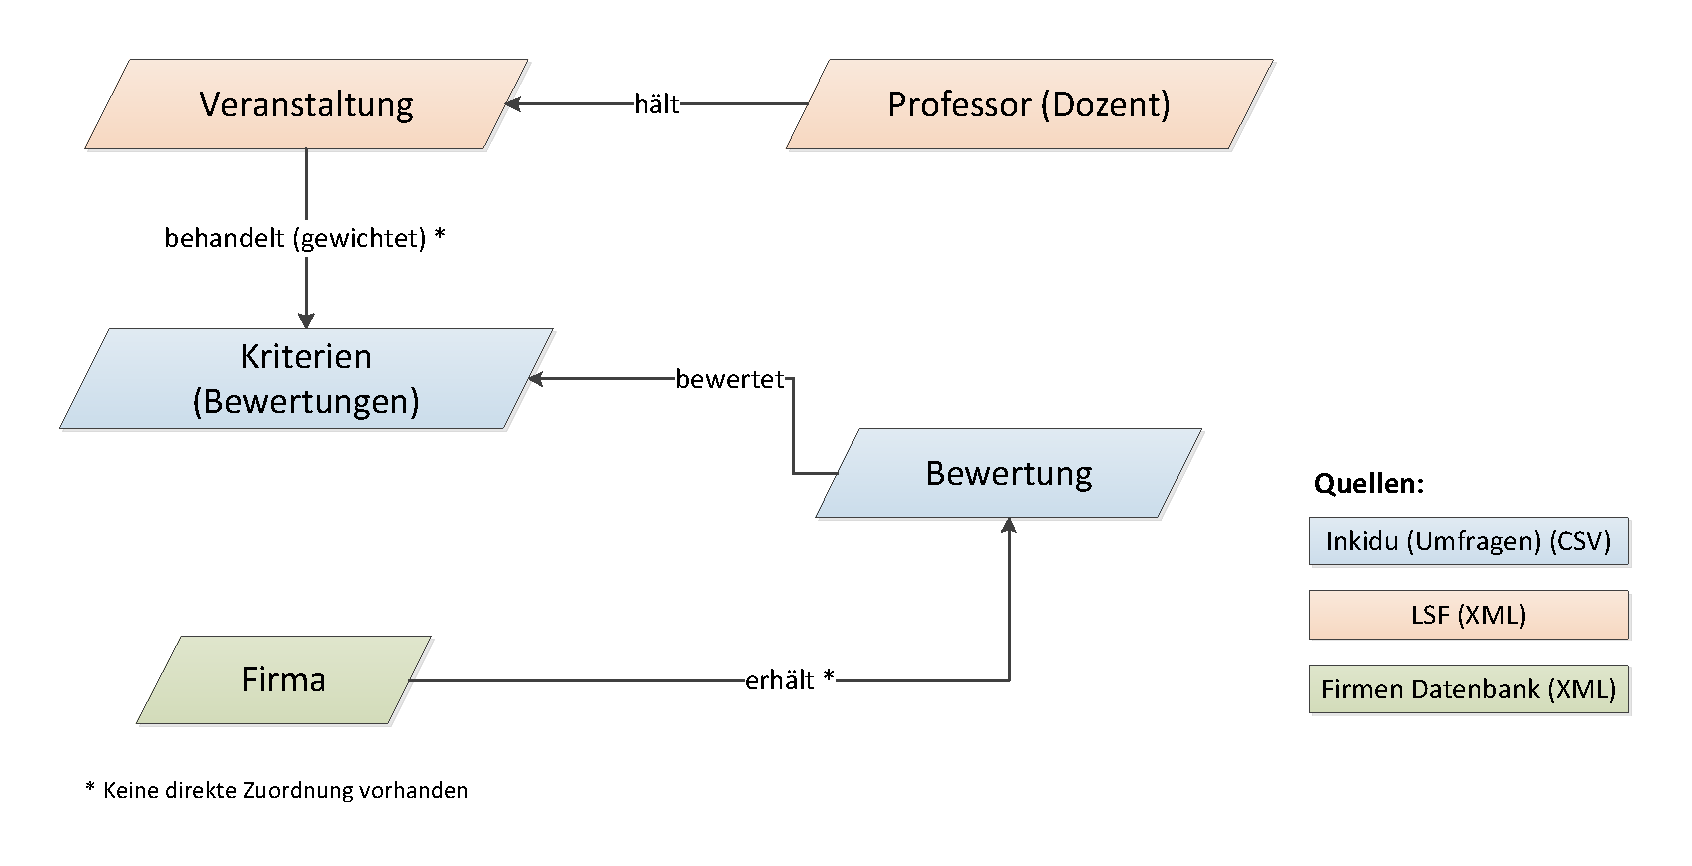
\includegraphics[scale=0.53]{images/Highlevel-Daten-Verkuepfung-Herkunft}
	\caption{Benötigte Daten und deren Beziehungen (vereinfacht)}
	\label{graphic-highlevel-data}
\end{figure}

Abbildung \ref{graphic-highlevel-data} zeigt die Daten und deren Beziehungen. In dieser stark vereinfachten Darstellung kann man die Zusammenhänge zwischen den Daten leicht erkennen. Auch deren Quellen, sowie das Format wird in der Grafik kurz angedeutet.

%\subsection{Datenquellen} %\subsection{Open Linked Data an der Hochschule}
Die Daten an der Hochschule über Veranstaltungen oder Professoren werden im sogenannten \gls{LSF} der Firma HIS verwaltet. Dabei werden einige Informationen auch öffentlich als HTML ausgeliefert. Leider werden diese Informationen nicht als Triples (z.B. in RDF) veröffentlicht. Es gibt lediglich auf Anfrage beim Rechenzentrum eine XML Schnittstelle bei der die benötigten Daten aus der Datenbank verfügbar gemacht werden können.


%\subsubsection{Formate und Konvertierung} % überflüssig???
Wie in Abbildung \ref{graphic-highlevel-data} bereits unter Quellen zu sehen, gibt es 3 primäre Datenquellen für unsere Anwendung an der Hochschule. Die mit * gekennzeichneten Verbindungen sind nicht vorhanden bzw. lassen sich nicht direkt aus den Daten ableiten.

\paragraph{LSF} Das LSF\footnote{\url{http://www.lsf.hs-weingarten.de}} bietet einen XML Export. Leider ist diese Schnittstelle noch nicht so weit ausgebaut als das wir sie für unser Projekt nutzen könnten. Daher wurden die LSF Daten exemplarisch von Hand ermittelt. Verbindungen zwischen Veranstaltung und Dozenten (Professoren) sind jedoch eindeutig.

\paragraph{Fimen Datenbank} Die Firmendatenbank (PDB) wird von Hand von der LeiterIn des Praktikantenamts gepflegt. Manuell werden die Daten als XML auf einem Webserver abgelegt.

\paragraph{INKIDU} Das Online Umfragesystem INKIDU\footnote{\url{http://inkidu.de}} ermöglicht einen \gls{CSV} Export der Umfrageergebnisse. Dieses System erlaubt dem Nutzer nur Freitextfelder und bietet daher keine Verbindung zwischen den Umfrageergebnissen und den Daten die zu einer Firma in der Firmendatenbank gespeichert sind. Ideen für die Zuordnung finden sich im Abschnitt \ref{sec-algo}.


\subsection{Algorithmen}
\label{sec-algo}
Um aus den Daten ``Linked Data'' zu machen, können verschiedene Techniken angewandt werden. Primär geht es darum, eine Zuordnung zwischen nicht direkt verbundenen Datensätzen zu finden. Ein weiterer Aspekt bei der Veröffentlichung von Daten ist der Datenschutz. Da es sich bei den Bewertungen um Meinungen von Studenten über Firmen handelt, dürfen diese natürlich nicht direkt veröffentlicht werden.

\subsubsection{Firmenzuordnung} % andreas
Wie bereits mehrfach erwähnt, gibt es keine Zuordnung zwischen den Firmen in der Firmen Datenbank und den Bewertungen der Studenten. Dadurch, dass die Daten in verschiedensten Formaten vorliegen und auch nicht in einem einheitlichen Konzept abgelegt wurden, bzw. keine eindeutige Identität haben, ist es nur möglich diese anhand eines Pattern-Matching-Verfahrens zu vergleichen und die größtmögliche Ähnlichkeit als Referenz zu verwenden.\\
Dabei wird ein String, der einen Firmennamen repräsentiert, anhand der im String vorkommenden einzelnen Worte unterteilt und dabei ausgehend von rechts nach links mit dem vorliegenden String verglichen. Wichtig ist dabei, dass unbedingt von rechts angefangen werden muss den String zu vergleichen, da in der deutschen Sprache Firmennamen immer mit der Gesellschaftsform am Ende definiert werden.
Nehmen wir einmal das Beispiel
\begin{verbatim}
 Mayer Informatik GmbH
\end{verbatim}
so würde dies maximal drei Durchläufe zum Vergleich ergeben:
\begin{verbatim}
 Mayer Informatik GmbH
 Mayer Informatik
 Mayer
\end{verbatim}
Dabei kann es natürlich passieren, dass zum Ergebnis \texttt{Mayer} mehrere Einträge in der Firmendatenbank gefunden werden, aber dies ist anhand der vorliegenden Daten leider nicht zu vermeiden. Ist nach dem dritten Durchlauf immer noch kein Matching möglich, so wird der Versuch erfolglos abgebrochen. In beiden Fällen wird die Firma im Ergebnis nicht angezeigt.

\subsubsection{Bayesian average}
Der CSV Export der INKIDU Umfragen enthält jede Firmenbewertung einzeln.
Aus Datenschutzgründen müssen diese Bewertungen vor der Veröffentlichung auf einen Wert pro Firma aggregiert werden.
Um eine faire Gewichtung zwischen Firmen mit vielen Bewertungen und welchen mit wenigen zu erreichen wird die ``Bayesian average'' (\ref{eq:bayesavg}) berechnet.

\begin{equation}
\bar{x} = {Cm + \sum_{i=1}^n{x_i} \over C + n} 	\label{eq:bayesavg}
\end{equation}

Hierbei ist $C$ die durchschnittliche Anzahl der Bewertungen, $m$ der A-priori Durchschnitt und $n$ die Anzahl der Bewertungen für dieses Element.
Eine praktische Erklärung ist in \cite{Weichs06} zu finden.

% Hier Nur Algos für die Datenkonvertierung KEINE für die eigentlich Anwendung!!!

\section{Datenmodellierung im Projekt} 	% war: Design des Projekts
\label{sec-idee-datenmodel}
\subsection{Ontologien}
Ziel beim Aufbau der Ontologie für unseren Anwendungsfall ist es, so viele standardisierte ``Terms'' zu verwenden wie möglich. Sich also stets bei anderen, bekannten und etablierten Ontologien zu bedienen.
Es soll nachher keine völlig neue Ontologie entstehen, sondern nur die Teile für die es keine ``Terms'' gibt erweitert werden. Im Sinne des Semantic Web Gedanken, sollten Daten wie Bezeichnungen von Objekten möglichst mit den bekannten Terms bezeichnet werden. 

In dem Vortrag von Tim Berners Lee vom Mai 2010  \cite{W3CQALD} greift er die Problematik der Zurückhaltung vieler Entwickler in Sachen Semantic Web auf. Viele Entwickler haben das Semantic Web missverstanden, prangert der Web-Erfinder an und versucht es anhand einer Tüte Kartoffelchips für jeden verständlich zu erklären. Es wird keine große universalgültige Ontologie geben, doch das darf uns nicht davon abhalten die Techniken nicht einzusetzen. \textit{Open Your Data NOW!}

Im Folgenden werden Ontologien, die wir im Projekt benutzt haben, vorgestellt:

\paragraph{DC}
Dublin Core\footnote{\url{http://dublincore.org}} beschreibt grundlegende Metadaten-Elemente. Die Elemente wie Titel, Ersteller, Thema, Beschreibung, Datum und Sprache sind allgemeingültig genug um viele Dinge wie Bücher, Filme, Bilder oder Web Seiten zu beschreiben.
Dublin Core ist auch als ISO Standard 15836 festgelegt.

\paragraph{FOAF}
\label{foaf}
Friend of a Friend\footnote{\url{http://www.foaf-project.org}} ermöglicht es Menschen und ihre Beziehungen untereinander maschinenlesbar darzustellen.
Dazu gehört zum einen Menschen zu beschreiben, also Eigenschaften wie Namen, Alter, Email Adresse und Website zu definieren.
Zum anderem werden Relationen zwischen Personen modelliert. Dies kann entweder über direkte ``knows'' Beziehung zwischen Menschen geschehen oder über Gruppenzugehörigkeiten.

Die Spezifikation\footnote{\url{http://xmlns.com/foaf/spec/}} wird stets weiterentwickelt und wurde zuletzt im Januar 2010 aktualisiert.
Viele soziale Netzwerke wie LiveJournal und identi.ca\footnote{\url{http://identi.ca}} bieten FOAF Informationen über ihre Nutzer an.
Daraus resultiert, dass FOAF einen Großteil der im Web verfügbaren semantischen Daten repräsentiert.
Auch in Zukunft wird FOAF eine wichtige Rolle spielen, wenn soziale Netzwerke via FOAF+SSL\footnote{\url{http://esw.w3.org/Foaf\%2Bssl}} oder mit Diaspora\footnote{\url{http://www.joindiaspora.com}} komplett dezentral werden.

\paragraph{AIISO}
Die \gls{AIISO}\footnote{\url{http://vocab.org/aiiso/schema}} ist eine Ontologie mit welcher die Struktur von akademischen Instituten beschrieben wird.
Es können Lehreinheiten wie Kurse, Fächer und Module beschrieben werden. Diese können, ganz im Sinne von Linked-Data, wiederum andere Lehreinheiten enthalten und auf diese verweisen.
Des weiteren können Fakultäten, Departments, Institute und ihre Zusammenhänge beschrieben werden.

\paragraph{SKOS}
\gls{SKOS}\footnote{\url{http://www.w3.org/2004/02/skos/}} ist ein einfaches \gls{KOS} für das Semantic Web.
Die vom W3C selbst entwickelte Spezifikation\footnote{\url{http://www.w3.org/TR/skos-reference/}} erlaubt es ein eigenes Vokabular zu veröffentlichten.
Somit ist es möglich Konzepte und Begriffe für ein Klassifizierungsschema oder eine Taxonomie zu definieren.

\paragraph{Eigene Definition}

\begin{figure}[htbp]
	\centering
	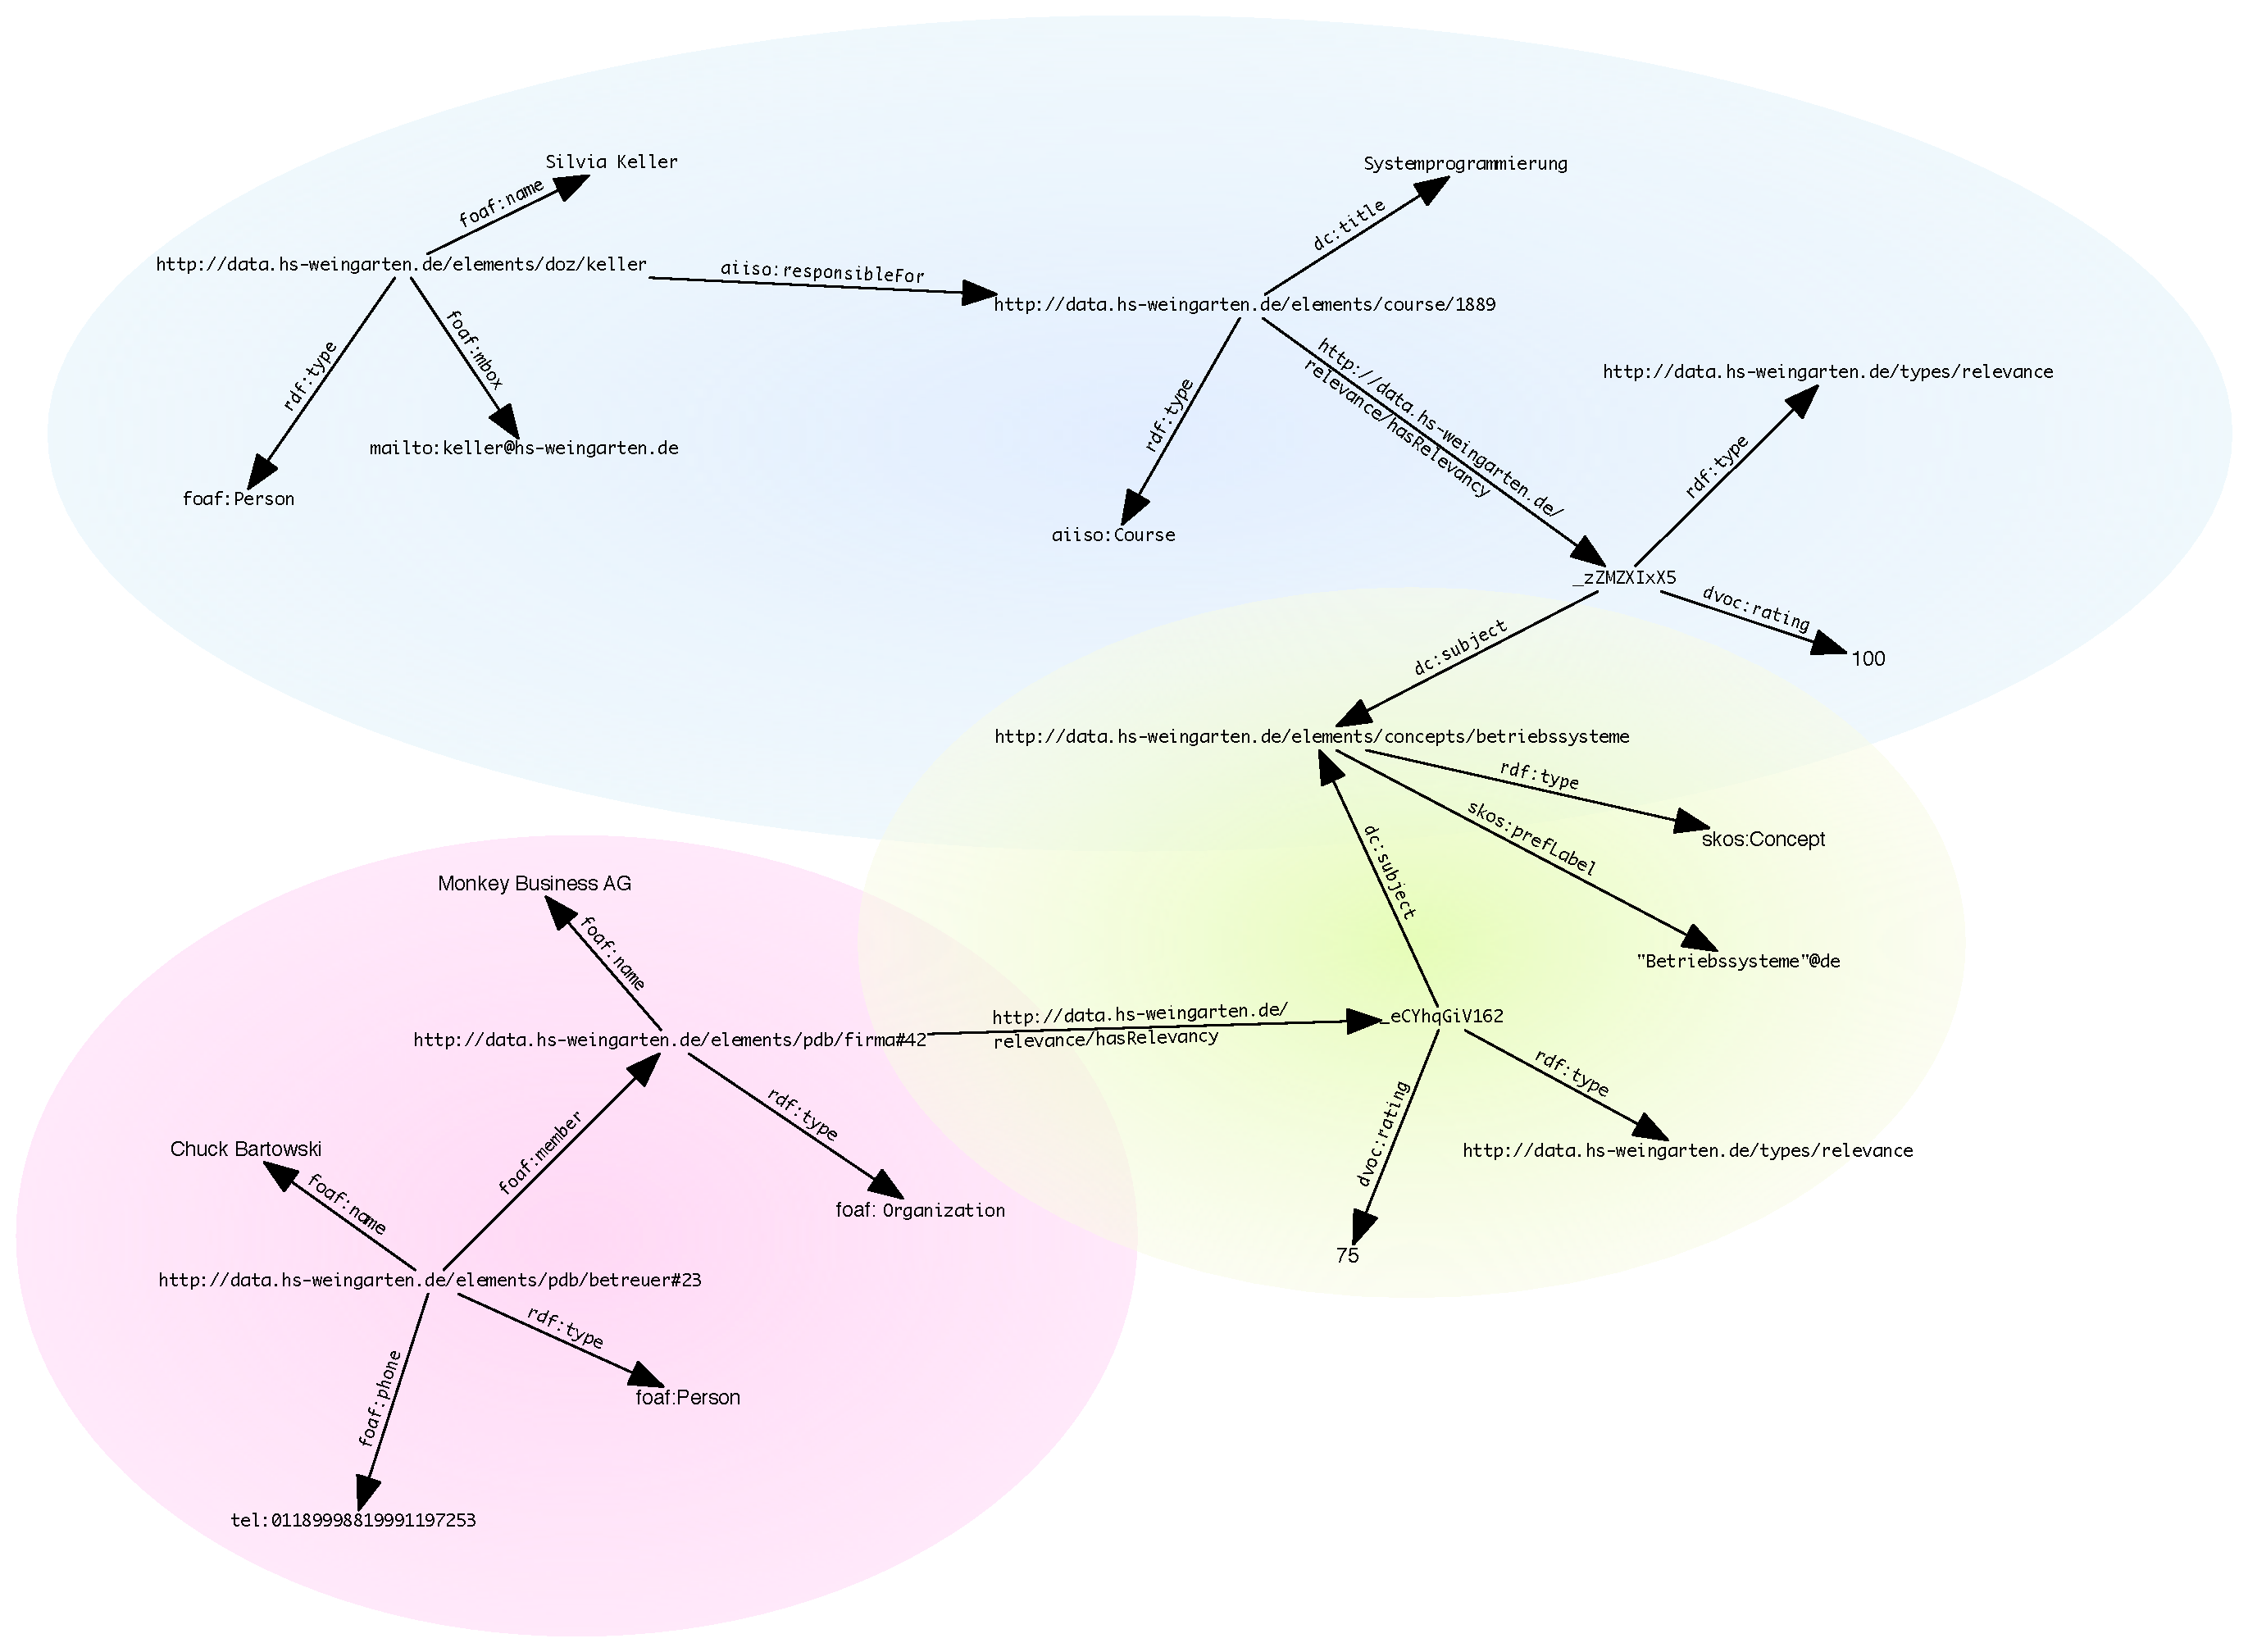
\includegraphics[scale=0.45,angle=90]{images/graph.pdf}
	\caption{Aufbau des Datenmodells an einem konkreten Beispiel}
	\label{example-graph}
\end{figure}

Ein Großteil der verwendeten Daten kann also mit bereits bestehenden Ontologien modelliert werden.
Einzig für die Relevanz-Information zwischen einem Topic (skos:Concept) und einem anderem Subjekt wurde ein eigenes Format definiert.
Die Zusammenhänge der Daten werden in Abbildung \ref{example-graph} verdeutlicht.

Es ist empfehlenswert bekannte und bereits bestehende Ontologien einzusetzen, da somit das Verbinden mehrerer Datenquellen vereinfacht wird.
Auch wenn dies keine harte Anforderung ist, da man mit ``owl:sameAs'' relativ einfach mappings zwischen unterschiedlichen Ontologien herstellen kann,
ist es dennoch sinnvoll auf bereits bestehenden Arbeiten aufzubauen.
Aus diesem Grund werden weitere Empfehlungen für Ontologien in \cite{ONTOPAT} aktiv mit der Community als Wiki diskutiert.
\newpage
\subsection{Daten veröffentlichen} 			% Data fetching / publishing
Die Daten werden als RDF Dateien auf einem Webserver abgelegt. Zusätzlich soll ein SPARQL Endpoint dafür sorgen, das jeder direkte Abfragen über Daten machen kann.

Die Subdomain ``data'' hat sich für die Veröffentlichung von (semantischen) Daten bewährt.
Prominente Beispiele:
\begin{itemize}
 \item \href{http://data.gov}{data.gov} - US Regierung
 \item \href{http://data.gov.uk}{data.gov.uk} - UK Regierung
 \item \href{http://data.worldbank.com}{data.worldbank.com} - Weltbank
 \item \href{http://data.nytimes.com}{data.nytimes.com} - New York Times
\end{itemize}

Daher wäre die Adresse \textbf{data.hs-weingarten.de} wünschenswert.

\section{Klassifizierung der Firmen und Professoren}		% Decision making by benny
\label{klassifizierung}
Sind alle Daten als ">Linked Data"< verfügbar, muss unsere Anwendung die Firmen und Professoren den gewählten Schwerpunkten und Präferenzen des Studenten zuordnen. Diese Zuordnung wird auch als \textbf{Klassifikationsproblem} bezeichnet. In \cite{Ertel08} finden sich im Kapitel 8 detaillierte Erklärungen zu den einzelnen Verfahren. 
Die erste Schwierigkeit ist ein geeignetes Verfahren für die Klassifizierung zu finden. Das Verfahren muss die größtmögliche Ähnlichkeit der Daten in der Datenbank, mit den eingegebenen Daten finden. Es orientiert sich an den bisherigen Daten (Bewertungen). Diese werden daher auch als Trainingsdaten bezeichnet.
\\
Ein einfaches Verfahren diese Ähnlichkeit zwischen den gegebenen und den gesuchten Daten zu finden, ist die Nearest-Neighbour-Klassifikation. Dabei werden beispielsweise mit Hilfe der euklidischen Distanz die Abstände zwischen dem gesuchten Punkt im n-dimensionalen Raum und den gespeicherten Punkten gesucht. Der neue Punkt wird dann gleich klassifiziert wie der Punkt der ihm am nächsten ist. In Abbildung \ref{graph-voronoi} ist in einem Voronoi-Diagramm dargestellt. Jeder Punkt wird von einem konvexen Polygon umgeben welches das Gebiet definiert, in dem ein neuer Punkt gleich diesem Punkt klassifiziert wird.
\begin{figure}[htbp]
	\centering
	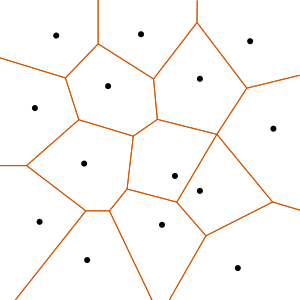
\includegraphics[keepaspectratio,scale=0.6]{images/Voronoi-Diagramm}
	\caption{Beispiel eines Voronoi-Diagramm}
	\label{graph-voronoi}
\end{figure}
\newpage
Das Problem dabei ist das durch Ausreißer, Rauschen oder Fehleingaben sich eine Überanpassung einstellen kann. In unserem Fall könnte eine sehr gute oder schlechte Bewertung die neue Bewertung stark beeinflussen und eine Firma ins Abseits schieben. Der k-Nearest-Neighbour-Algorithmus ist eine Verbesserung, die nicht nur den nächsten Nachbarn sondern die k nächsten Nachbarn betrachtet. Für k=3 also die 3 nächsten Nachbarn.

Der beschriebene Algorithmus (inkl. Verbesserung) zählt zu den \textit{lazy learning} (faules Lernen) Verfahren, weil bei der Berechnung immer alle Trainingsdaten benutzt werden. Dies ist bei kleinen Datenmengen jedoch unkritisch.

% % Raus weil wir das nicht machen, und wir auch nicht wirklich den nn-algo nutzen!! (karl)

%Aus diesem Grund verwenden wir den k-Nearest-Neighbour-Algorithmus zur Klassifikation. Dieser betrachtet nicht nur einen Punkt aus der Menge  sondern die seine K Nachbarn mit minimalem Abstand. Problematisch wird dabei aber das weiter entfernte Punkte meist die direkten Nachbarn dominieren. Um dies zu verhindern, werden die k-Nachbarn gewichtet. Die Punkte werden nun mit dem Gewicht
%\begin{equation}
%\omega_i = {1 \over d(x,x_{i})^2} 	\label{eq:AbstandkNN}
%\end{equation}
%das quadratisch mit dem Abstand abnimmt, gewichtet.











%
% Umsetzung
%
\chapter{Umsetzung}
\label{cap-umsetzung}
Dieser Abschnitt beschreibt die technischen Hilfsmittel und Vorgehensweisen bei der Umsetzung der Projektidee.
Die Architektur kann in drei Bereiche geteilt werden.
Zuerst werden die Daten aus verschiedenen Quellen zusammengetragen, aufbereitet und in dem zentralen Triplestore gespeichert. (Siehe \ref{design-step11})
Der zweite Bereich beschäftigt sich damit, wie die semantischen Daten der Welt zugänglich gemacht werden.
Zuletzt wird die Beispielanwendung ``Semantic Internship Advisor'' vorgestellt, welcher auf die Daten zugreift.
\section{Architektur Übersicht}

\begin{figure}[h]
	\centering
	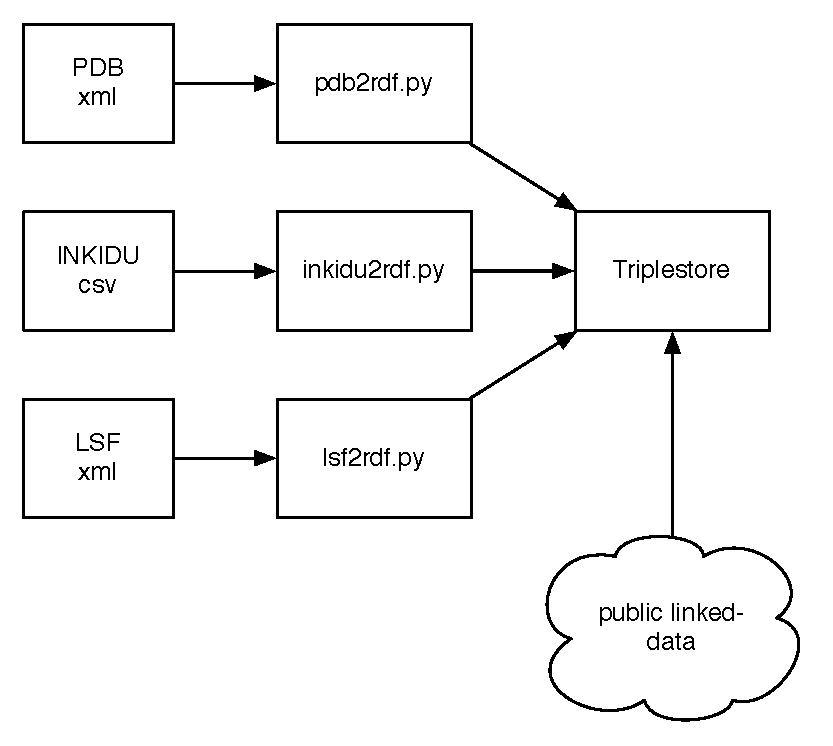
\includegraphics[scale=0.6,]{images/step1_1.pdf}
	\caption{Architektur: Daten aufbereiten}
	\label{design-step11}
\end{figure}

\section{Daten aufbereiten: Python Skripte} %wiedi
\label{sec-daten-python}
Die Konvertierung der Datenquellen nach RDF ist mit Hilfe von drei kleinen Python Skripten umgesetzt.
Für jede Datenquelle wurde ein Skript verfasst.


\subsection{RDFLib}
\label{subsec-rdflib}
Dank RDFLib\footnote{\url{http://www.rdflib.net/}} ist das Erstellen eines Graphen und die Ausgabe als RDF/XML sehr einfach zu realisieren.
RDFLib ist eine Python Bibliothek, welche Parser und Serialisierer für viele Varianten von RDF enthält.
Des weiteren ist ein ``in-memory'' Graphstore enthalten. Es besteht aber ebenso die Möglichkeit den Graphen persistent zu speichern.

\subsection{Arbeitsweise}
Die Skripte arbeiten in zwei schritten.
Im ersten Schritt werden die Originaldaten geladen und in eine interne Datenstruktur gebracht.
Für XML Quellen wird das Python Modul ">xml.dom.minidom"< als Parser eingesetzt.
Für das CSV Format bietet Python in seiner Standardbibliothek einen Parser.

Im zweiten Schritt wird die Datenstruktur abgearbeitet und in Triples strukturiert.
Diese Triples werden dann in einen temporären Graphen eingefügt.

\begin{lstlisting}[language=Python,caption=Alle Betreuer einer Firma werden zum Graphen ``g'' hinzugefügt,stepnumber=1,label=umsetzung-rdflib-add]
for betreuer in firma['betreuer']:
	betreuer_node = PDB_BETREUER[betreuer['id']]
	g.add((betreuer_node, RDF.type, FOAF['Person']))
	g.add((betreuer_node, FOAF['member'], firma_node))
	g.add((betreuer_node, FOAF['name'], Literal(betreuer['name'])))
\end{lstlisting}

Im Codelisting \ref{umsetzung-rdflib-add} wird für jeden Betreuer einer Firma eine ``betreuer\_node'' im Namespace PDB\_BETREUER erstellt.
Über diese Node werden dann drei Aussagen (Triples) getroffen. Zuerst wird der Typ als foaf:Person festgelegt.
In Zeile 4 wird festgelegt, dass der Betreuer Mitglied einer Firma ist. Zuletzt wird der Name als Literal gesetzt.
Diese drei Aussagen werden in den Graphen ``g'' mit der ``add'' Methode hinzugefügt.

\subsection{Verknüpfen der Datenquellen}

In dem Umfragetool INKIDU werden die Firmen einzig über ein Freitextfeld identifiziert, welches vom Umfrageteilnehmer ausgefüllt wird.
Herauszufinden für welche Firma aus der PDB eine Bewertung gilt ist somit maschinell nicht trivial.

Das PDB Skript generiert für jede Firma eine eindeutige URI.
Während dem Konvertieren der INKIDU Daten wird versucht die URI der Firma zu finden.
Dazu wird dem Freitextfeld nur das erste Wort entnommen.
Darauf hin wird eine SPARQL Abfrage auf die konvertierten PDB Daten gestartet.
Da SPARQL Abfragen reguläre Ausdrücke enthalten können ist es möglich sehr mächtiges Stringmatching durchzuführen.

\begin{lstlisting}[language=Python,caption=Funktion um mit Hilfe von SPARQL Firma zu finden,stepnumber=1,label=umsetzung-firma-sparql]
def get_firma(haystack):
	sparql = SPARQLWrapper(SPARQL_ENDPOINT)
	sparql.setQuery("""
		PREFIX foaf:    <http://xmlns.com/foaf/0.1/>
		PREFIX rdf:     <http://www.w3.org/1999/02/22-rdf-syntax-ns#>
		SELECT ?firma
		WHERE { 
			?firma foaf:name ?firma_name .
			?firma rdf:type foaf:Organization .
			FILTER regex(?firma_name, "^%s", "i" )
		}
	""" % (haystack.split()[0], ))
	sparql.setReturnFormat(JSON)
	results = sparql.query().convert()['results']['bindings']
	if len(results) == 1:
		return results[0]['firma']['value']
	return None
\end{lstlisting}

In Listing \ref{umsetzung-firma-sparql} ist eine Funktion gezeigt, welche die eben beschriebene Vorgehensweise implementiert.
Zuerst wird eine SPAQRL-Verbindung zur Endpoint-URL aufgebaut.
Die Anfrage definiert zwei Namespaces.
Der Friend-of-a-Friend (siehe \ref{foaf}) Namespace wird als ``foaf'' abgekürzt. Ebenso wird der RDF Namespace festgelegt.
Gesucht wird eine Firma deren Name mit dem ersten Wort des Freitextfeldes beginnt und die vom Typ ``foaf:Organisation'' ist.
Kann diese Anfrage eindeutig beantwortet werden wird der Identifier zurückgegeben.


\section{Daten verfügbar machen: Jena und Joseki} % karl
\label{sec-daten-joseki}
Bei \textbf{Jena}\footnote{\url{http://openjena.org/}} handelt es sich um ein Framework für das Semantic Web in der Programmiersprache Java. Diese wurde ursprünglich in den ">HP Labs Semantic Web Research"<\footnote{\url{http://www.hpl.hp.com/semweb/}} entwickelt und ist seit Oktober 2009 ein unabhängiges Open-Source Projekt. Es ermöglicht, ähnlich wie die RDFLib (\ref{subsec-rdflib}), das bequeme lesen und schreiben von RDF Dateien. Darüber hinaus bietet Jena auch einen SPARQL Query-Endpoint (Server) namens \textbf{Joseki}. Alle Module in Jena sind so implementiert, dass die Teile auch einzeln zur Entwicklung einer eigenen Anwendung genutzt werden können.

\begin{figure}[h]
	\centering
	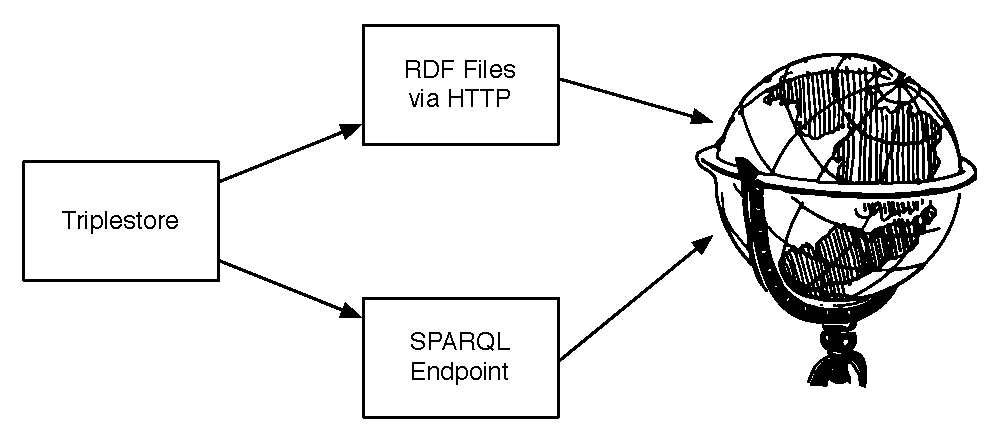
\includegraphics[scale=0.6,]{images/step1_2.pdf}
	\caption{Architektur: Daten veröffentlichen}
	\label{design-step12}
\end{figure}

\subsection{Joseki Server}
Die Joseki Web-Anwendung stellt das zentrale Element unseres Servers dar. Es erfüllt die Aufgabe, die gesammelten Daten dem gesamten Web bereit zu stellen. Unsere Anwendung (siehe \ref{cap-projektidee} und \ref{sec-our-app}) ist nur eine von vielen möglichen Anwendungen die diese Daten dann nutzen kann.

Da wir die Daten sowohl als statische RDF-Dateien zum Download, also auch über das SPARQL-Protokoll anbieten, werden die HTTP Verbindungen von einem Apache Webserver angenommen.
So werden die statischen Dateien, sowie die Beispiel-Webanwendung vom Apache ausgeliefert.
Stellt der Webserver anhand der aufgerufenen URL fest,
dass es sich um eine SPARQL Abfrage handelt, wird die Verbindung an den Joseki Server weitergegeben.

%\todo[inline]{Kurz die Config erklären, N3 usw. vielleicht auch die Storage Engines erwähnen?!}
%\todo[inline]{data.hs-weingarten.de ?? Oder erst in Fazit?}

\section{Die Anwendung: Semantic Internship Advisor}
\label{sec-our-app}

Die Anwendung wurde komplett in JavaScript realisiert. Dazu werden die beiden Bibliotheken ">jQuery"<\footnote{\url{http://jquery.com}} und ">sparql.js"< verwendet. Die Anwendung macht direkte Abfragen auf den Joseki SPARQL Endpoint (siehe \ref{sec-daten-joseki}).
Beim Aufruf der Anwendung werden die Themen und Schwerpunkte über eine SPARQL Abfrage geladen und daraus dynamisch eine HTML Form aufgebaut.
Hat der Benutzer seine Schwerpunkte und Präferenzen festgelegt werden die Firmen, die am ehesten dazu passen geladen und inklusive möglichen Betreuern angezeigt.

\paragraph{Abfragen}
In Listing \ref{umsetzung-app-sparql} ist zu sehen wie eine SPARQL Abfrage unter JavaScript aussehen kann.
In diesem Beispiel wird zuerst ein SPARQL Objekt mit dem Endpoint als Parameter angelegt.
Daraufhin werden wie üblich die verwendeten Namespaces deklariert.
In Zeile 7 wird das eigentliche Query ausgeführt, wobei wie in JavaScript üblich die Callback-Handler inline als Parameter angegeben werden.
Bei Erfolg (Zeile 13) kann die Antwort verarbeitet werden. Hier werden die einzelnen Schwerpunkte als Option in ein Auswahlfeld hinzugefügt.

\begin{lstlisting}[language=JavaScript,caption=SPARQL Abfrage mit JavaScript,stepnumber=1,label=umsetzung-app-sparql]
var s = new SPARQL.Service("http://fh-data.frubar.net/query/hswgt");
s.setPrefix("rdf", "http://www.w3.org/1999/02/22-rdf-syntax-ns#")
s.setPrefix("aiiso", "http://purl.org/vocab/aiiso/schema#")
s.setPrefix("dc", "http://purl.org/dc/elements/1.1/")

var q = s.createQuery();
q.query("SELECT ?m ?title FROM <http://fh-data.frubar.net/rdf/lsf.rdf> \
             WHERE { ?m rdf:type aiiso:Programme . ?m dc:title ?title }",
  {
    failure: function() {
      alert('Laden der Schwerpunkte fehlgeschlagen');
    },
    success: function(json) {
      for (var x in json.results.bindings) {
        $('#schwerpunkt').append($("<option></option>").
          attr("value",json.results.bindings[x].m.value).
          text(json.results.bindings[x].title.value));
      }
    }
  });
\end{lstlisting}

Folgende (geplante) Eigenschaften sind nicht implementiert:
\begin{itemize}
 \item Vorschlag eines Betreuers (Professor) pro Firma
 \item Daten vom LSF werden nicht verarbeitet
 \item Kein automatisches Laden von INKIDU Umfrageergebnissen
 \item Kein durchstöbern (browsen) der Daten möglich
% \item Keine LSF Integration der der Anwendung (als LSF-Modul)
\end{itemize}
Die Daten vom LSF konnten uns im Zeithorizont des Projektes leider Aufgrund von fehlenden Kapazitäten im Rechenzentrum nicht bereitgestellt werden.

\paragraph{Zuordnung} Die Zuordnung von Firmen zu den gewählten Schwerpunkten ist aus mehreren Gründen nicht wie in \ref{graphic-highlevel-data} beschreiben realisiert worden:
\begin{itemize}
 \item Keine ">echten"< Daten aus dem LSF.
 \item Fehlende Bewertung der Kriterien pro Veranstaltung
\end{itemize}

Aus diesen Gründen wurde für die Demo-Anwendung die Schwerpunkte direkt mit Kriterien (in der Anwendung Präferenzen genannt) bewertet. Diese Bewertung wurde von uns ">nach Gefühl"< vorgenommen.

Die Bewertungen werden aufgrund der in Abschnitt \ref{sec-algo} kurz angesprochenen Datenschutzbedenken nicht direkt veröffentlicht, sondern als ein Mittelwert. Daher wird auch nicht direkt der in \ref{klassifizierung} vorgestellte Nearest Neighbour Algorithmus verwendet. Das Prinzip ist zwar das selbe, jedoch gibt es für jede Klasse (entspricht Firma) nur einen Trainingsdatensatz. Somit werden diese nur aufsteigend nach den Abständen sortiert.

\begin{figure}[htbp]
	\centering
	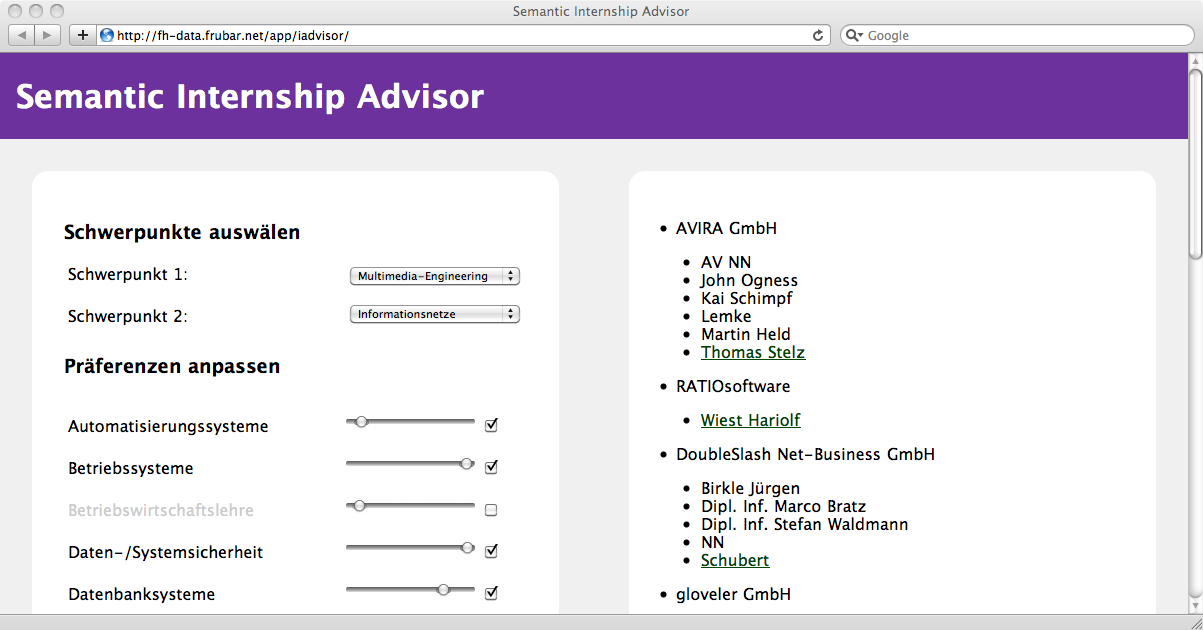
\includegraphics[scale=0.39]{images/sia.png}
	\caption{Screenshot der Anwendung }
	\label{sia-screenshot}
\end{figure}


\subsection{Semantische Benutzeroberflächen}
Da Semantic Web Anwendungen meist datenorientierter als herkömmliche Webanwendungen sind, sollten die Userinterface Möglichkeiten ebenfalls neu überdacht werden.
Für den Semantic Internship Advisor wird deshalb ein neues HTML5 Slider-Element verwendet um die Präferenzen einzustellen.
\begin{lstlisting}[language=HTML,caption=HTML 5 Slider,stepnumber=1,label=umsetzung-html5-slider]
<input type="range" />
\end{lstlisting}
Eine ausführlichere Betrachtung des Themas bietet \cite{Aufr08}.
Mit SMILE\footnote{\url{http://www.simile-widgets.org/}} gibt es bereits eine eigene Widget-Bibliothek für das Semantic Web.

Eine sehr frühe Demo-Version unserer Anwendung ist unter \url{http://fh-data.frubar.net/app/iadvisor/} zu finden.

\subsection{Mögliche Erweiterungen}

\paragraph{Maps} Es könnte z.B. aus den vorhandenen Adressdaten direkt ein Map-Widget eingebunden werden. APIs für diesen Zweck gibt es sowohl vom freien OpenStreetMaps (siehe Abbildung \ref{osm-screenshot}) als auch von Google.

\paragraph{Weitere Firmeninformationen} Es wäre denkbar über Freebase oder DBPedia (\ref{dbpedia}) Informationen wie ">Anzahl der Mitarbeiter"< abzufragen. Dabei gibt es nur ein Zuordnungsproblem. Gemäß dem Linked Data Ansatz müssten unsere RDFs eigentlich ein \textit{owl:sameAs} mit einer Referenz auf den Eintrag in z.B. DBPedia haben. Da wir diese Informationen jedoch nicht manuell nachtragen möchten, würde sich hier eine Suche nach Firmenname anbieten. SPARQL hilft dabei jedoch nicht, denn eine Freitextsuche ist hier (zumindest im Allgemeinen) nicht möglich. Es gibt jedoch Dienste wie \href{lookup.dbpedia.org}{http://lookup.dbpedia.org} die so etwas ermöglichen.

\begin{figure}[htbp]
	\centering
	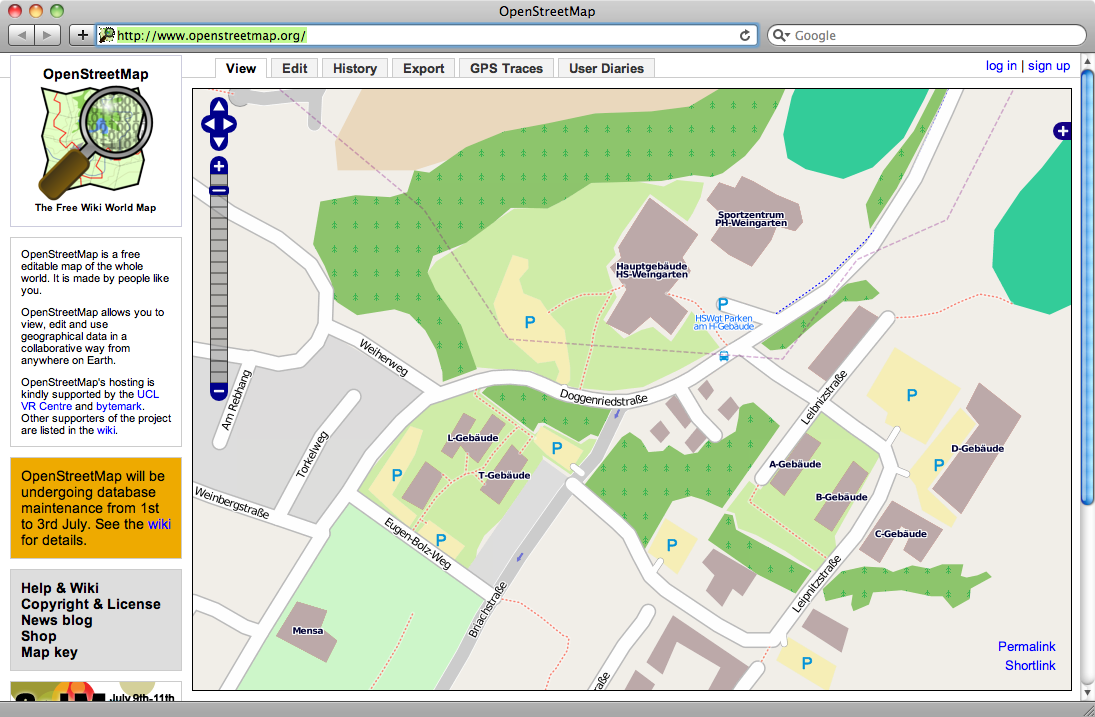
\includegraphics[scale=0.39]{images/osm-shot.png}
	\caption{OpenStreetMap Beispiel}
	\label{osm-screenshot}
\end{figure}


 


%
% Zusammenfassung
%
\chapter{Zusammenfassung}
\label{cap-zusafa}

%\todo[inline]{In einleitung schauen was hier genau hinkommt...}

\section{Fazit}
\label{sec-fazit}
Die Erfahrungen mit der vom Team erstellten Anwendung zeigt deutlich, dass es zwar ungewohnt, jedoch nicht allzu kompliziert ist, Daten semantisch aufzubereiten und zu verarbeiten. Anwendungsentwicklung mit Semantic Web Techniken ist einfach und kann viel Spaß bereiten. Alle Projektteilnehmer haben viel gelernt.

Positiv überrascht wurden wir durch die Flexibilität und Kooperationsbereitschaft verschiedener Instanzen.
Hierbei möchten wir uns noch einmal beim Rechenzentrum der HS-Weingarten und Marius Ebel vom INKIDU-Team für die Zusammenarbeit bedanken. Das Rechenzentrum hat uns den, für die Entwicklung den nötigen (virtuellen) Server, bereitgestellt. Hierfür möchten wir uns ebenfalls bedanken.

Aufgrund des kurzen zeitlichem Rahmens dieser Arbeit konnten leider nicht alle Ziele erreicht werden.
Auf die Daten des LSF System mussten wir leider verzichten, da der Export vom Rechenzentrum so kurzfristig nicht umgesetzt werden konnte.

Ebenso konnten wir die in dieser Arbeit erstellten Daten nur über Umwege veröffentlichen.
Die sehr restriktiven Firewall-Regeln des Rechenzentrums erschwerten das Bereitstellen der Anwendung unter der Internet-Adresse der Hochschule und war nur über einen externen Proxy möglich.


%  vielleicht anderer Algorithmus zur Bewertung/Ergebnisberechung da Klassifizierungs algorithmen für viele klasse ineffizient werden -> gründ ertel buch S. 198 -> kleinste Quadrate usw.
\section{Ausblick}
\label{sec-ausblick}
Ein Ziel für zukünftige Semantic Web Projekte an der Hochschule Ravensburg-Weingarten muss sein, das Angebot an Daten zu erhöhen und diese bereitzustellen. Vor allem sollten Daten direkt aus dem LSF exportiert werden, da es sich bei dieser Anwendung um die zentrale Dokumentationsquelle aller relevanten Daten der Organisationsstruktur der Hochschule handelt.\\
Würde die Hochschule einen zentrales System für semantische Datenverarbeitung bereitstellen, welcher z.B. unter data.hs-weingarten.de auch aus dem Internet erreichbar ist, so könnte man alle gewünschten Daten semantisch aufbereitet der Öffentlichkeit zur Verfügung stellen. Zudem wäre die Hochschule hier ein Vorreiter in der Nutzung von semantischen Web-Techniken und dies würde langfristig dazu führen, dass zum einen weitere Forschungsprojekte, gegebenenfalls auch aus der Industrie, entstehen, welche auch Geld für selbige mitbringen. Zudem würde es den Ruf der Hochschule, gerade im Bereich Informatik nochmals erhöhen und langfristig auch dafür sorgen, dass andere Hochschulen und Universitäten in Daten semantisch veröffentlichen. Aus diesen Daten, welche dann deutschlandweit von allen Hochschulen existieren ließen sich dann Vergleiche anstellen, Rankings generieren uvm. Den Möglichkeiten sind hier sogut wie keine Grenzen gesetzt.\\
Ein weiterer Aspekt dieser Veröffentlichung wäre, dass dann jeder auf Basis dieser Daten eigene Anwendungen erstellen kann, die z.B. den Studenten das Studium vereinfachen.

Das Projekt ist als OpenSource Projekt im Web\footnote{\url{https://frucman.frubar.net/info-xml/}} verfügbar. Interessierte können an dem Projekt auch nach Ablauf der Projektphase teilhaben.




%\part{Anhang}

%Glossar ausgeben
%\addcontentsline{toc}{chapter}{Glossar}
\printglossary[style=altlist,title=Glossar]
\newpage
%\todo[inline]{Verzeichnisse (Abbildung und Tables: ans laufen bekommen!!!)}
\listoffigures
\listoftables
\lstlistoflistings
\newpage
\begin{thebibliography}{wasweissich}

	\bibitem[Bern01]{Bern01} Tim Berners-Lee, James Hendler, Ora Lassila \flqq {\sl The Semantic Web: a new form of Web content that is meaningful to computers will unleash a revolution of new possibilities. In: Scientific American, 284 (5), S. 34–43, May 2001}\frqq
	\url{http://www.scientificamerican.com/article.cfm?id=the-semantic-web}


\bibitem[Sega09]{Sega09} Toby Segaran, Colin Evans, and Jamie Taylor \flqq {\sl Programming the Semantic Web}\frqq

\bibitem[Ertel08]{Ertel08} Wolfgang Ertel \flqq {\sl Grundkurs Künstliche Intelligenz } \frqq \url{http://www.hs-weingarten.de/~ertel/kibuch}

\bibitem[XML03]{XML03} H. Wittenbrink, W. Köhler, O. Bergmann et al. \flqq {\sl XML. SPC TEIA Lehrbuch Verlag, Berlin, 2003. ISBN 3-935539-69-X}\frqq


\bibitem[Aufr08]{Aufr08} Michael Aufreiter \flqq {\sl Informationsvisualisierung und Navigation im Semantic Web: Eine Analyse bestehender Visualisierungstechniken im Hinblick auf Eignung für das Semantic Web} \frqq \url{http://quasipartikel.at/wp-content/uploads/2009/05/informationsvisualisierung_im_semantic-web1.pdf}


\end{thebibliography}

%\cite{dadada}
% -> [test]

%\cite{test1}
% -> [1]


\newpage
\renewcommand{\refname}{Weblinks}
\begin{thebibliography}{wasweissich}

\bibitem[RDF-Prim]{RDF-Prim} Frank Manola, Eric Miller \flqq {\sl RDF Primer W3C Recommendation 10 February 2004, besucht am 29.06.2010} \frqq
	\url{http://www.w3.org/TR/rdf-primer/}
	
\bibitem[WATSON]{WATSON} \flqq {\sl WATSON Ontologie Suchmaschine für das Semantic Web, besucht am 29.06.2010} \frqq \url{http://watson.kmi.open.ac.uk/}
	
\bibitem[W3SRDF]{W3SRDF} \flqq {\sl W3Schools Tutorial zu RDF, besucht am 29.06.2010} \frqq \url{http://www.w3schools.com/rdf/rdf_main.asp/}

\bibitem[ONTOPAT]{ONTOPAT} \flqq {\sl Ontology Design Patterns} \frqq \url{http://ontologydesignpatterns.org/}

\bibitem[W3CQALD]{W3CQALD} Tim Berners-Lee \flqq {\sl Linked data: It's is not like that; it's like a bag of potato chips.} \frqq \url{http://www.w3.org/QA/2010/05/linked_data_its_is_not_like_th.html}

\bibitem[WPSEMWEB]{WPSEMWEB} \flqq {\sl Wikipeida: Semantisches Web} \frqq \url{http://de.wikipedia.org/wiki/Semantisches_Web}

\bibitem[LINKEDATA]{LINKEDATA} \flqq {\sl  A home for, or pointers to, resources from across the Linked Data community} \frqq \url{http://linkeddata.org/}

\bibitem[Weichs06]{Weichs06} Markus Weichselbaum \flqq {\sl Bayesian Rating - how to implement a weighted rating system} \frqq \url{http://www.thebroth.com/blog/118/bayesian-rating} 

\bibitem[Kred07]{Kred07} Heinz Kredel \flqq {\sl Metadaten: DC, RDF und OWL 2007, besucht am 29.06.2010} \frqq \url{http://krum.rz.uni-mannheim.de/inet-2007/sess-308.html} 

\bibitem[OWL09]{OWL09} Michael K. Smith,Chris Welty, Deborah L. McGuinness \flqq {\sl OWL Web Ontology Language Guide, Deutsche Übersetzung, besucht am 29.06.2010} \frqq \url{http://www.semaweb.org/dokumente/w3/TR/2004/REC-owl-guide-20040210-DE.html}
\end{thebibliography}

%\cite{dadada}
% -> [test]

%\cite{test1}
% -> [1]


\end{document}
